% Options for packages loaded elsewhere
% Options for packages loaded elsewhere
\PassOptionsToPackage{unicode}{hyperref}
\PassOptionsToPackage{hyphens}{url}
\PassOptionsToPackage{dvipsnames,svgnames,x11names}{xcolor}
%
\documentclass[
  11pt,
]{article}
\usepackage{xcolor}
\usepackage[margin=1in]{geometry}
\usepackage{amsmath,amssymb}
\setcounter{secnumdepth}{-\maxdimen} % remove section numbering
\usepackage{iftex}
\ifPDFTeX
  \usepackage[T1]{fontenc}
  \usepackage[utf8]{inputenc}
  \usepackage{textcomp} % provide euro and other symbols
\else % if luatex or xetex
  \usepackage{unicode-math} % this also loads fontspec
  \defaultfontfeatures{Scale=MatchLowercase}
  \defaultfontfeatures[\rmfamily]{Ligatures=TeX,Scale=1}
\fi
\usepackage{lmodern}
\ifPDFTeX\else
  % xetex/luatex font selection
\fi
% Use upquote if available, for straight quotes in verbatim environments
\IfFileExists{upquote.sty}{\usepackage{upquote}}{}
\IfFileExists{microtype.sty}{% use microtype if available
  \usepackage[]{microtype}
  \UseMicrotypeSet[protrusion]{basicmath} % disable protrusion for tt fonts
}{}
\makeatletter
\@ifundefined{KOMAClassName}{% if non-KOMA class
  \IfFileExists{parskip.sty}{%
    \usepackage{parskip}
  }{% else
    \setlength{\parindent}{0pt}
    \setlength{\parskip}{6pt plus 2pt minus 1pt}}
}{% if KOMA class
  \KOMAoptions{parskip=half}}
\makeatother
% Make \paragraph and \subparagraph free-standing
\makeatletter
\ifx\paragraph\undefined\else
  \let\oldparagraph\paragraph
  \renewcommand{\paragraph}{
    \@ifstar
      \xxxParagraphStar
      \xxxParagraphNoStar
  }
  \newcommand{\xxxParagraphStar}[1]{\oldparagraph*{#1}\mbox{}}
  \newcommand{\xxxParagraphNoStar}[1]{\oldparagraph{#1}\mbox{}}
\fi
\ifx\subparagraph\undefined\else
  \let\oldsubparagraph\subparagraph
  \renewcommand{\subparagraph}{
    \@ifstar
      \xxxSubParagraphStar
      \xxxSubParagraphNoStar
  }
  \newcommand{\xxxSubParagraphStar}[1]{\oldsubparagraph*{#1}\mbox{}}
  \newcommand{\xxxSubParagraphNoStar}[1]{\oldsubparagraph{#1}\mbox{}}
\fi
\makeatother

\usepackage{color}
\usepackage{fancyvrb}
\newcommand{\VerbBar}{|}
\newcommand{\VERB}{\Verb[commandchars=\\\{\}]}
\DefineVerbatimEnvironment{Highlighting}{Verbatim}{commandchars=\\\{\}}
% Add ',fontsize=\small' for more characters per line
\usepackage{framed}
\definecolor{shadecolor}{RGB}{241,243,245}
\newenvironment{Shaded}{\begin{snugshade}}{\end{snugshade}}
\newcommand{\AlertTok}[1]{\textcolor[rgb]{0.68,0.00,0.00}{#1}}
\newcommand{\AnnotationTok}[1]{\textcolor[rgb]{0.37,0.37,0.37}{#1}}
\newcommand{\AttributeTok}[1]{\textcolor[rgb]{0.40,0.45,0.13}{#1}}
\newcommand{\BaseNTok}[1]{\textcolor[rgb]{0.68,0.00,0.00}{#1}}
\newcommand{\BuiltInTok}[1]{\textcolor[rgb]{0.00,0.23,0.31}{#1}}
\newcommand{\CharTok}[1]{\textcolor[rgb]{0.13,0.47,0.30}{#1}}
\newcommand{\CommentTok}[1]{\textcolor[rgb]{0.37,0.37,0.37}{#1}}
\newcommand{\CommentVarTok}[1]{\textcolor[rgb]{0.37,0.37,0.37}{\textit{#1}}}
\newcommand{\ConstantTok}[1]{\textcolor[rgb]{0.56,0.35,0.01}{#1}}
\newcommand{\ControlFlowTok}[1]{\textcolor[rgb]{0.00,0.23,0.31}{\textbf{#1}}}
\newcommand{\DataTypeTok}[1]{\textcolor[rgb]{0.68,0.00,0.00}{#1}}
\newcommand{\DecValTok}[1]{\textcolor[rgb]{0.68,0.00,0.00}{#1}}
\newcommand{\DocumentationTok}[1]{\textcolor[rgb]{0.37,0.37,0.37}{\textit{#1}}}
\newcommand{\ErrorTok}[1]{\textcolor[rgb]{0.68,0.00,0.00}{#1}}
\newcommand{\ExtensionTok}[1]{\textcolor[rgb]{0.00,0.23,0.31}{#1}}
\newcommand{\FloatTok}[1]{\textcolor[rgb]{0.68,0.00,0.00}{#1}}
\newcommand{\FunctionTok}[1]{\textcolor[rgb]{0.28,0.35,0.67}{#1}}
\newcommand{\ImportTok}[1]{\textcolor[rgb]{0.00,0.46,0.62}{#1}}
\newcommand{\InformationTok}[1]{\textcolor[rgb]{0.37,0.37,0.37}{#1}}
\newcommand{\KeywordTok}[1]{\textcolor[rgb]{0.00,0.23,0.31}{\textbf{#1}}}
\newcommand{\NormalTok}[1]{\textcolor[rgb]{0.00,0.23,0.31}{#1}}
\newcommand{\OperatorTok}[1]{\textcolor[rgb]{0.37,0.37,0.37}{#1}}
\newcommand{\OtherTok}[1]{\textcolor[rgb]{0.00,0.23,0.31}{#1}}
\newcommand{\PreprocessorTok}[1]{\textcolor[rgb]{0.68,0.00,0.00}{#1}}
\newcommand{\RegionMarkerTok}[1]{\textcolor[rgb]{0.00,0.23,0.31}{#1}}
\newcommand{\SpecialCharTok}[1]{\textcolor[rgb]{0.37,0.37,0.37}{#1}}
\newcommand{\SpecialStringTok}[1]{\textcolor[rgb]{0.13,0.47,0.30}{#1}}
\newcommand{\StringTok}[1]{\textcolor[rgb]{0.13,0.47,0.30}{#1}}
\newcommand{\VariableTok}[1]{\textcolor[rgb]{0.07,0.07,0.07}{#1}}
\newcommand{\VerbatimStringTok}[1]{\textcolor[rgb]{0.13,0.47,0.30}{#1}}
\newcommand{\WarningTok}[1]{\textcolor[rgb]{0.37,0.37,0.37}{\textit{#1}}}

\usepackage{longtable,booktabs,array}
\usepackage{calc} % for calculating minipage widths
% Correct order of tables after \paragraph or \subparagraph
\usepackage{etoolbox}
\makeatletter
\patchcmd\longtable{\par}{\if@noskipsec\mbox{}\fi\par}{}{}
\makeatother
% Allow footnotes in longtable head/foot
\IfFileExists{footnotehyper.sty}{\usepackage{footnotehyper}}{\usepackage{footnote}}
\makesavenoteenv{longtable}
\usepackage{graphicx}
\makeatletter
\newsavebox\pandoc@box
\newcommand*\pandocbounded[1]{% scales image to fit in text height/width
  \sbox\pandoc@box{#1}%
  \Gscale@div\@tempa{\textheight}{\dimexpr\ht\pandoc@box+\dp\pandoc@box\relax}%
  \Gscale@div\@tempb{\linewidth}{\wd\pandoc@box}%
  \ifdim\@tempb\p@<\@tempa\p@\let\@tempa\@tempb\fi% select the smaller of both
  \ifdim\@tempa\p@<\p@\scalebox{\@tempa}{\usebox\pandoc@box}%
  \else\usebox{\pandoc@box}%
  \fi%
}
% Set default figure placement to htbp
\def\fps@figure{htbp}
\makeatother





\setlength{\emergencystretch}{3em} % prevent overfull lines

\providecommand{\tightlist}{%
  \setlength{\itemsep}{0pt}\setlength{\parskip}{0pt}}



 


\makeatletter
\@ifpackageloaded{caption}{}{\usepackage{caption}}
\AtBeginDocument{%
\ifdefined\contentsname
  \renewcommand*\contentsname{Table of contents}
\else
  \newcommand\contentsname{Table of contents}
\fi
\ifdefined\listfigurename
  \renewcommand*\listfigurename{List of Figures}
\else
  \newcommand\listfigurename{List of Figures}
\fi
\ifdefined\listtablename
  \renewcommand*\listtablename{List of Tables}
\else
  \newcommand\listtablename{List of Tables}
\fi
\ifdefined\figurename
  \renewcommand*\figurename{Figure}
\else
  \newcommand\figurename{Figure}
\fi
\ifdefined\tablename
  \renewcommand*\tablename{Table}
\else
  \newcommand\tablename{Table}
\fi
}
\@ifpackageloaded{float}{}{\usepackage{float}}
\floatstyle{ruled}
\@ifundefined{c@chapter}{\newfloat{codelisting}{h}{lop}}{\newfloat{codelisting}{h}{lop}[chapter]}
\floatname{codelisting}{Listing}
\newcommand*\listoflistings{\listof{codelisting}{List of Listings}}
\makeatother
\makeatletter
\makeatother
\makeatletter
\@ifpackageloaded{caption}{}{\usepackage{caption}}
\@ifpackageloaded{subcaption}{}{\usepackage{subcaption}}
\makeatother
\usepackage{bookmark}
\IfFileExists{xurl.sty}{\usepackage{xurl}}{} % add URL line breaks if available
\urlstyle{same}
\hypersetup{
  pdftitle={Unemployment and Voter Turnout Analysis},
  pdfauthor={Statistical Analysis - STA 702},
  colorlinks=true,
  linkcolor={blue},
  filecolor={Maroon},
  citecolor={Blue},
  urlcolor={Blue},
  pdfcreator={LaTeX via pandoc}}


\title{Unemployment and Voter Turnout Analysis}
\usepackage{etoolbox}
\makeatletter
\providecommand{\subtitle}[1]{% add subtitle to \maketitle
  \apptocmd{\@title}{\par {\large #1 \par}}{}{}
}
\makeatother
\subtitle{Research Question 1: How does local Unemployment tier relate
to voter turnout?}
\author{Statistical Analysis - STA 702}
\date{2025-12-10}
\begin{document}
\maketitle

\renewcommand*\contentsname{Table of contents}
{
\hypersetup{linkcolor=}
\setcounter{tocdepth}{3}
\tableofcontents
}

\begin{center}\rule{0.5\linewidth}{0.5pt}\end{center}

\section{\texorpdfstring{\textbf{Theoretical Motivation - Political
Participation
Framework}}{Theoretical Motivation - Political Participation Framework}}\label{theoretical-motivation---political-participation-framework}

Political theory suggests that populations differ in their typical level
of political engagement. Almond and Verba's classic ``Civic Culture''
framework describes a participation pyramid in which the largest group
consists of disengaged citizens (``parochials''), followed by moderately
involved voters (``subjects''), and finally a small group of highly
engaged participants.

In many systems, this bottom tier, often described as a ``silent
majority'', remains politically inactive unless economic or social
conditions deteriorate. Under worsening economic conditions, previously
uninvolved citizens may become mobilized to vote, either to punish the
incumbent or express dissatisfaction with the status quo.

This idea motivates our investigation of whether local Unemployment
tiers, measured through rising unemployment, affect the incumbent
party's electoral performance at the county level.\\
\strut \\
Almond, Gabriel A., and Sidney Verba.~\emph{The Civic Culture: Political
Attitudes and Democracy in Five Nations.}~Princeton University Press,
1963

Berelson, Bernard R., Paul F. Lazarsfeld, and William N.
McPhee.~\emph{Voting: A Study of Opinion Formation in a Presidential
Campaign.}~University of Chicago Press, 1954.

\begin{Shaded}
\begin{Highlighting}[]
\FunctionTok{library}\NormalTok{(ggplot2)}
\FunctionTok{library}\NormalTok{(dplyr)}

\CommentTok{\# Data: three layers of the participation pyramid}
\NormalTok{pyramid\_df }\OtherTok{\textless{}{-}} \FunctionTok{tibble}\NormalTok{(}
  \AttributeTok{level =} \FunctionTok{factor}\NormalTok{(}\FunctionTok{c}\NormalTok{(}\StringTok{"Participants"}\NormalTok{, }\StringTok{"Subjects"}\NormalTok{, }\StringTok{"Parochials"}\NormalTok{), }
                 \AttributeTok{levels =} \FunctionTok{c}\NormalTok{(}\StringTok{"Participants"}\NormalTok{, }\StringTok{"Subjects"}\NormalTok{, }\StringTok{"Parochials"}\NormalTok{)),}
  \AttributeTok{ymin =} \FunctionTok{c}\NormalTok{(}\FloatTok{0.66}\NormalTok{, }\FloatTok{0.33}\NormalTok{, }\DecValTok{0}\NormalTok{),}
  \AttributeTok{ymax =} \FunctionTok{c}\NormalTok{(}\DecValTok{1}\NormalTok{, }\FloatTok{0.66}\NormalTok{, }\FloatTok{0.33}\NormalTok{),}
  \AttributeTok{label =} \FunctionTok{c}\NormalTok{(}
    \StringTok{"Participants:}\SpecialCharTok{\textbackslash{}n}\StringTok{Highly engaged voters;}\SpecialCharTok{\textbackslash{}n}\StringTok{consistent political activity"}\NormalTok{,}
    \StringTok{"Subjects:}\SpecialCharTok{\textbackslash{}n}\StringTok{Moderately engaged;}\SpecialCharTok{\textbackslash{}n}\StringTok{responsive in major elections"}\NormalTok{,}
    \StringTok{"Parochials:}\SpecialCharTok{\textbackslash{}n}\StringTok{Low engagement;}\SpecialCharTok{\textbackslash{}n}\StringTok{\textquotesingle{}Silent Majority\textquotesingle{}}\SpecialCharTok{\textbackslash{}n}\StringTok{activated by crises"}
\NormalTok{  )}
\NormalTok{)}

\CommentTok{\# Base triangle shape}
\NormalTok{triangle }\OtherTok{\textless{}{-}} \FunctionTok{data.frame}\NormalTok{(}
  \AttributeTok{x =} \FunctionTok{c}\NormalTok{(}\FloatTok{0.5}\NormalTok{, }\DecValTok{1}\NormalTok{, }\DecValTok{0}\NormalTok{),}
  \AttributeTok{y =} \FunctionTok{c}\NormalTok{(}\DecValTok{1}\NormalTok{, }\DecValTok{0}\NormalTok{, }\DecValTok{0}\NormalTok{)}
\NormalTok{)}

\FunctionTok{ggplot}\NormalTok{() }\SpecialCharTok{+}
  \CommentTok{\# Triangle outline}
  \FunctionTok{geom\_polygon}\NormalTok{(}\AttributeTok{data =}\NormalTok{ triangle, }\FunctionTok{aes}\NormalTok{(x, y), }\AttributeTok{fill =} \StringTok{"white"}\NormalTok{, }\AttributeTok{color =} \StringTok{"black"}\NormalTok{) }\SpecialCharTok{+}
  
  \CommentTok{\# Layers inside the triangle}
  \FunctionTok{geom\_rect}\NormalTok{(}\AttributeTok{data =}\NormalTok{ pyramid\_df, }
            \FunctionTok{aes}\NormalTok{(}\AttributeTok{xmin =} \DecValTok{0}\NormalTok{, }\AttributeTok{xmax =} \DecValTok{1}\NormalTok{, }\AttributeTok{ymin =}\NormalTok{ ymin, }\AttributeTok{ymax =}\NormalTok{ ymax, }\AttributeTok{fill =}\NormalTok{ level),}
            \AttributeTok{alpha =} \FloatTok{0.6}\NormalTok{, }\AttributeTok{color =} \StringTok{"black"}\NormalTok{) }\SpecialCharTok{+}
  
  \CommentTok{\# Descriptive text inside each layer}
  \FunctionTok{geom\_text}\NormalTok{(}\AttributeTok{data =}\NormalTok{ pyramid\_df,}
            \FunctionTok{aes}\NormalTok{(}\AttributeTok{x =} \FloatTok{0.5}\NormalTok{, }\AttributeTok{y =}\NormalTok{ (ymin }\SpecialCharTok{+}\NormalTok{ ymax) }\SpecialCharTok{/} \DecValTok{2}\NormalTok{, }\AttributeTok{label =}\NormalTok{ label),}
            \AttributeTok{color =} \StringTok{"black"}\NormalTok{, }\AttributeTok{size =} \DecValTok{4}\NormalTok{, }\AttributeTok{lineheight =} \DecValTok{1}\NormalTok{,}
            \AttributeTok{fontface =} \StringTok{"bold"}\NormalTok{) }\SpecialCharTok{+}
  
  \FunctionTok{scale\_fill\_manual}\NormalTok{(}\AttributeTok{values =} \FunctionTok{c}\NormalTok{(}
    \StringTok{"Participants"} \OtherTok{=} \StringTok{"\#6fa8dc"}\NormalTok{,}
    \StringTok{"Subjects"} \OtherTok{=} \StringTok{"\#9fc5e8"}\NormalTok{,}
    \StringTok{"Parochials"} \OtherTok{=} \StringTok{"\#cfe2f3"}
\NormalTok{  )) }\SpecialCharTok{+}
  
  \FunctionTok{coord\_fixed}\NormalTok{() }\SpecialCharTok{+}
  \FunctionTok{theme\_void}\NormalTok{() }\SpecialCharTok{+}
  \FunctionTok{theme}\NormalTok{(}
    \AttributeTok{legend.position =} \StringTok{"none"}\NormalTok{,}
    \AttributeTok{plot.title =} \FunctionTok{element\_text}\NormalTok{(}\AttributeTok{size =} \DecValTok{16}\NormalTok{, }\AttributeTok{face =} \StringTok{"bold"}\NormalTok{, }\AttributeTok{hjust =} \FloatTok{0.5}\NormalTok{)}
\NormalTok{  ) }\SpecialCharTok{+}
  \FunctionTok{ggtitle}\NormalTok{(}\StringTok{"Political Participation Pyramid"}\NormalTok{)}
\end{Highlighting}
\end{Shaded}

\pandocbounded{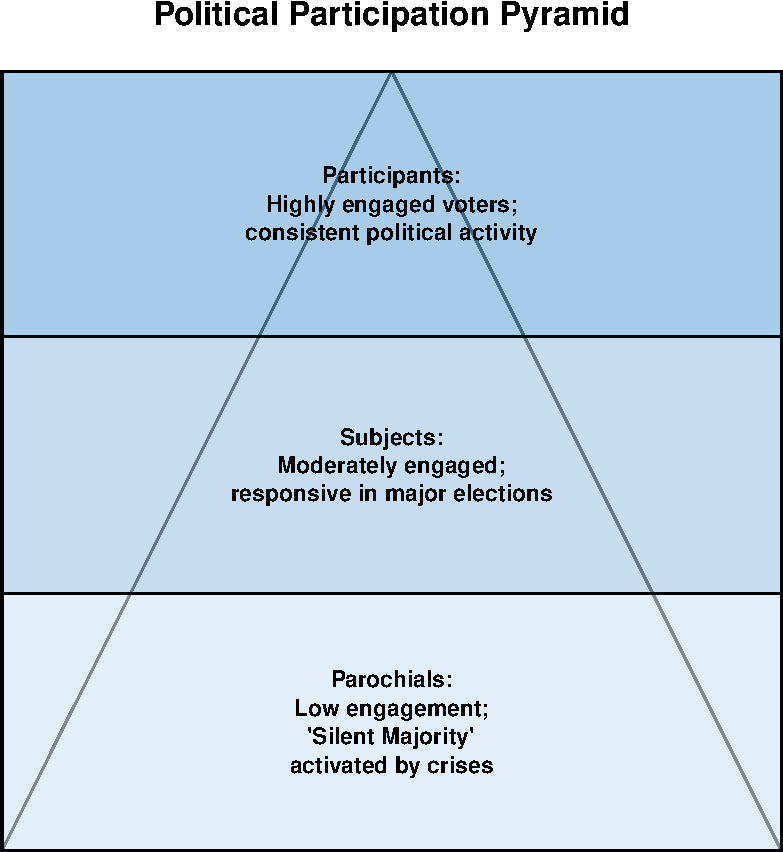
\includegraphics[keepaspectratio]{RQ1_v2_files/figure-pdf/unnamed-chunk-1-1.pdf}}

\begin{center}\rule{0.5\linewidth}{0.5pt}\end{center}

\section{Introduction}\label{introduction}

This analysis investigates the relationship between local economic
conditions (measured by unemployment rate) and voter turnout in U.S.
presidential and midterm elections from 2004-2022. Our data comes from
the Inter-university Consortium for Political and Social Research
(ICPSR) and the Bureau of Labor Statistics.

\textbf{Research Question:} How does local unemployment relate to voter
turnout in U.S. elections at the county level?

\textbf{Key Measures:}

\begin{itemize}
\tightlist
\item
  \textbf{Outcome:} County-level voter turnout rate (proportion of
  eligible voters who voted)
\item
  \textbf{Predictor:} County unemployment rate (annual average, \%)
\item
  \textbf{Interaction:} Unemployment effect by county type (Urban,
  Suburban, or Rural)
\end{itemize}

\begin{center}\rule{0.5\linewidth}{0.5pt}\end{center}

\section{Data Preparation}\label{data-preparation}

\begin{Shaded}
\begin{Highlighting}[]
\CommentTok{\# Load required packages}
\FunctionTok{library}\NormalTok{(tidyverse)}
\FunctionTok{library}\NormalTok{(lfe)           }\CommentTok{\# For fixed effects regression}
\FunctionTok{library}\NormalTok{(stargazer)     }\CommentTok{\# For regression tables}
\FunctionTok{library}\NormalTok{(ggplot2)}
\FunctionTok{library}\NormalTok{(knitr)}
\FunctionTok{library}\NormalTok{(gridExtra)}

\CommentTok{\# Set ggplot theme}
\FunctionTok{theme\_set}\NormalTok{(}\FunctionTok{theme\_minimal}\NormalTok{(}\AttributeTok{base\_size =} \DecValTok{12}\NormalTok{))}
\end{Highlighting}
\end{Shaded}

\begin{Shaded}
\begin{Highlighting}[]
\CommentTok{\# Load the merged dataset}
\NormalTok{df }\OtherTok{\textless{}{-}} \FunctionTok{read\_csv}\NormalTok{(}\StringTok{"../data/processed/merged\_voting\_unemployment\_complete.csv"}\NormalTok{,}
               \AttributeTok{show\_col\_types =} \ConstantTok{FALSE}\NormalTok{)}

\CommentTok{\# Display data structure}
\FunctionTok{cat}\NormalTok{(}\StringTok{"Dataset Overview:}\SpecialCharTok{\textbackslash{}n}\StringTok{"}\NormalTok{)}
\end{Highlighting}
\end{Shaded}

\begin{verbatim}
Dataset Overview:
\end{verbatim}

\begin{Shaded}
\begin{Highlighting}[]
\FunctionTok{cat}\NormalTok{(}\StringTok{"Observations:"}\NormalTok{, }\FunctionTok{nrow}\NormalTok{(df), }\StringTok{"}\SpecialCharTok{\textbackslash{}n}\StringTok{"}\NormalTok{)}
\end{Highlighting}
\end{Shaded}

\begin{verbatim}
Observations: 30912 
\end{verbatim}

\begin{Shaded}
\begin{Highlighting}[]
\FunctionTok{cat}\NormalTok{(}\StringTok{"Counties:"}\NormalTok{, }\FunctionTok{length}\NormalTok{(}\FunctionTok{unique}\NormalTok{(df}\SpecialCharTok{$}\NormalTok{FIPS)), }\StringTok{"}\SpecialCharTok{\textbackslash{}n}\StringTok{"}\NormalTok{)}
\end{Highlighting}
\end{Shaded}

\begin{verbatim}
Counties: 3103 
\end{verbatim}

\begin{Shaded}
\begin{Highlighting}[]
\FunctionTok{cat}\NormalTok{(}\StringTok{"Years:"}\NormalTok{, }\FunctionTok{min}\NormalTok{(df}\SpecialCharTok{$}\NormalTok{YEAR), }\StringTok{"{-}"}\NormalTok{, }\FunctionTok{max}\NormalTok{(df}\SpecialCharTok{$}\NormalTok{YEAR), }\StringTok{"}\SpecialCharTok{\textbackslash{}n}\StringTok{"}\NormalTok{)}
\end{Highlighting}
\end{Shaded}

\begin{verbatim}
Years: 2004 - 2022 
\end{verbatim}

\begin{Shaded}
\begin{Highlighting}[]
\FunctionTok{cat}\NormalTok{(}\StringTok{"Variables:"}\NormalTok{, }\FunctionTok{ncol}\NormalTok{(df), }\StringTok{"}\SpecialCharTok{\textbackslash{}n}\StringTok{"}\NormalTok{)}
\end{Highlighting}
\end{Shaded}

\begin{verbatim}
Variables: 21 
\end{verbatim}

\textbf{Data Cleaning}

\begin{Shaded}
\begin{Highlighting}[]
\CommentTok{\# Clean the dataset}
\NormalTok{df }\OtherTok{\textless{}{-}}\NormalTok{ df}\SpecialCharTok{\%\textgreater{}\%}
  \FunctionTok{filter}\NormalTok{(}
\NormalTok{    VOTER\_TURNOUT\_PCT }\SpecialCharTok{\textgreater{}} \DecValTok{0}\NormalTok{,           }\CommentTok{\# Drop zero turnout}
    \SpecialCharTok{!}\FunctionTok{is.na}\NormalTok{(VOTER\_TURNOUT\_PCT),       }\CommentTok{\# Drop missing turnout}
    \SpecialCharTok{!}\FunctionTok{is.na}\NormalTok{(unemployment\_rate),        }\CommentTok{\# Drop missing unemployment}
\NormalTok{    VOTER\_TURNOUT\_PCT }\SpecialCharTok{\textless{}=} \FloatTok{1.0}         \CommentTok{\# Sanity check: turnout ≤ 100\%}
\NormalTok{  )}

\FunctionTok{cat}\NormalTok{(}\StringTok{"CLEANED DATASET}\SpecialCharTok{\textbackslash{}n}\StringTok{"}\NormalTok{)}
\end{Highlighting}
\end{Shaded}

\begin{verbatim}
CLEANED DATASET
\end{verbatim}

\begin{Shaded}
\begin{Highlighting}[]
\FunctionTok{cat}\NormalTok{(}\StringTok{"===============}\SpecialCharTok{\textbackslash{}n}\StringTok{"}\NormalTok{)}
\end{Highlighting}
\end{Shaded}

\begin{verbatim}
===============
\end{verbatim}

\begin{Shaded}
\begin{Highlighting}[]
\FunctionTok{cat}\NormalTok{(}\StringTok{"Observations remaining:"}\NormalTok{, }\FunctionTok{nrow}\NormalTok{(df), }\StringTok{"}\SpecialCharTok{\textbackslash{}n}\StringTok{"}\NormalTok{)}
\end{Highlighting}
\end{Shaded}

\begin{verbatim}
Observations remaining: 29769 
\end{verbatim}

\subsection{Variable Creation}\label{variable-creation}

\begin{Shaded}
\begin{Highlighting}[]
\DocumentationTok{\#\# Variable Creation}
\NormalTok{df }\OtherTok{\textless{}{-}}\NormalTok{ df }\SpecialCharTok{\%\textgreater{}\%}
  \FunctionTok{mutate}\NormalTok{(}
    \CommentTok{\# Election type indicator}
    \AttributeTok{is\_presidential =} \FunctionTok{ifelse}\NormalTok{(YEAR }\SpecialCharTok{\%\%} \DecValTok{4} \SpecialCharTok{==} \DecValTok{0}\NormalTok{, }\DecValTok{1}\NormalTok{, }\DecValTok{0}\NormalTok{),}
    \AttributeTok{election\_type =} \FunctionTok{ifelse}\NormalTok{(is\_presidential }\SpecialCharTok{==} \DecValTok{1}\NormalTok{, }\StringTok{"Presidential"}\NormalTok{, }\StringTok{"Midterm"}\NormalTok{),}
    
    \CommentTok{\# Unemployment tiers based on standard deviations from mean}
    \AttributeTok{unemp\_mean =} \FunctionTok{mean}\NormalTok{(unemployment\_rate, }\AttributeTok{na.rm =} \ConstantTok{TRUE}\NormalTok{),}
    \AttributeTok{unemp\_sd =} \FunctionTok{sd}\NormalTok{(unemployment\_rate, }\AttributeTok{na.rm =} \ConstantTok{TRUE}\NormalTok{),}
    
    \CommentTok{\# Calculate z{-}score}
    \AttributeTok{unemp\_zscore =}\NormalTok{ (unemployment\_rate }\SpecialCharTok{{-}}\NormalTok{ unemp\_mean) }\SpecialCharTok{/}\NormalTok{ unemp\_sd,}
    
    \CommentTok{\# Create tier classifications}
    \AttributeTok{unemployment\_tier =} \FunctionTok{case\_when}\NormalTok{(}
\NormalTok{      unemp\_zscore }\SpecialCharTok{\textless{}} \SpecialCharTok{{-}}\FloatTok{1.0} \SpecialCharTok{\textasciitilde{}} \StringTok{"Very Low (\textless{} {-}1 SD)"}\NormalTok{,}
\NormalTok{      unemp\_zscore }\SpecialCharTok{\textless{}} \SpecialCharTok{{-}}\FloatTok{0.5} \SpecialCharTok{\textasciitilde{}} \StringTok{"Low ({-}1 to {-}0.5 SD)"}\NormalTok{,}
\NormalTok{      unemp\_zscore }\SpecialCharTok{\textless{}} \FloatTok{0.5}  \SpecialCharTok{\textasciitilde{}} \StringTok{"Medium ({-}0.5 to 0.5 SD)"}\NormalTok{,}
\NormalTok{      unemp\_zscore }\SpecialCharTok{\textless{}} \FloatTok{1.0}  \SpecialCharTok{\textasciitilde{}} \StringTok{"High (0.5 to 1 SD)"}\NormalTok{,}
      \ConstantTok{TRUE}                \SpecialCharTok{\textasciitilde{}} \StringTok{"Very High (\textgreater{} 1 SD)"}
\NormalTok{    ),}
    
    \CommentTok{\# Ordered factor for modeling}
    \AttributeTok{unemployment\_tier =} \FunctionTok{factor}\NormalTok{(unemployment\_tier, }
                              \AttributeTok{levels =} \FunctionTok{c}\NormalTok{(}\StringTok{"Very Low (\textless{} {-}1 SD)"}\NormalTok{, }
                                        \StringTok{"Low ({-}1 to {-}0.5 SD)"}\NormalTok{,}
                                        \StringTok{"Medium ({-}0.5 to 0.5 SD)"}\NormalTok{,}
                                        \StringTok{"High (0.5 to 1 SD)"}\NormalTok{,}
                                        \StringTok{"Very High (\textgreater{} 1 SD)"}\NormalTok{),}
                              \AttributeTok{ordered =} \ConstantTok{TRUE}\NormalTok{),}
    
    \CommentTok{\# Standardized variables}
    \AttributeTok{unemployment\_std =}\NormalTok{ (unemployment\_rate }\SpecialCharTok{{-}} \FunctionTok{mean}\NormalTok{(unemployment\_rate)) }\SpecialCharTok{/} 
                       \FunctionTok{sd}\NormalTok{(unemployment\_rate),}
    
    \CommentTok{\# Urban/rural classification based on CVAP}
    \AttributeTok{county\_type =} \FunctionTok{case\_when}\NormalTok{(}
\NormalTok{      CVAP }\SpecialCharTok{\textgreater{}} \DecValTok{50000} \SpecialCharTok{\textasciitilde{}} \StringTok{"Urban"}\NormalTok{,}
\NormalTok{      CVAP }\SpecialCharTok{\textgreater{}} \DecValTok{10000} \SpecialCharTok{\textasciitilde{}} \StringTok{"Suburban"}\NormalTok{,}
      \ConstantTok{TRUE} \SpecialCharTok{\textasciitilde{}} \StringTok{"Rural"}
\NormalTok{    ),}
    
    \CommentTok{\# Factor variables for regression}
    \AttributeTok{FIPS\_factor =} \FunctionTok{as.factor}\NormalTok{(FIPS),}
    \AttributeTok{YEAR\_factor =} \FunctionTok{as.factor}\NormalTok{(YEAR),}
    \AttributeTok{STATE\_factor =} \FunctionTok{as.factor}\NormalTok{(STATE\_FIPS)}
\NormalTok{  )}

\CommentTok{\# Summary of unemployment tier distribution}
\FunctionTok{cat}\NormalTok{(}\StringTok{"✓ Created classification variables}\SpecialCharTok{\textbackslash{}n}\StringTok{"}\NormalTok{)}
\end{Highlighting}
\end{Shaded}

\begin{verbatim}
✓ Created classification variables
\end{verbatim}

\begin{Shaded}
\begin{Highlighting}[]
\FunctionTok{cat}\NormalTok{(}\StringTok{"  {-} Mean unemployment:"}\NormalTok{, }\FunctionTok{round}\NormalTok{(df}\SpecialCharTok{$}\NormalTok{unemp\_mean[}\DecValTok{1}\NormalTok{], }\DecValTok{2}\NormalTok{), }\StringTok{"\%}\SpecialCharTok{\textbackslash{}n}\StringTok{"}\NormalTok{)}
\end{Highlighting}
\end{Shaded}

\begin{verbatim}
  - Mean unemployment: 5.95 %
\end{verbatim}

\begin{Shaded}
\begin{Highlighting}[]
\FunctionTok{cat}\NormalTok{(}\StringTok{"  {-} SD unemployment:"}\NormalTok{, }\FunctionTok{round}\NormalTok{(df}\SpecialCharTok{$}\NormalTok{unemp\_sd[}\DecValTok{1}\NormalTok{], }\DecValTok{2}\NormalTok{), }\StringTok{"\%}\SpecialCharTok{\textbackslash{}n\textbackslash{}n}\StringTok{"}\NormalTok{)}
\end{Highlighting}
\end{Shaded}

\begin{verbatim}
  - SD unemployment: 2.67 %
\end{verbatim}

\begin{Shaded}
\begin{Highlighting}[]
\FunctionTok{cat}\NormalTok{(}\StringTok{"Distribution of unemployment tiers:}\SpecialCharTok{\textbackslash{}n}\StringTok{"}\NormalTok{)}
\end{Highlighting}
\end{Shaded}

\begin{verbatim}
Distribution of unemployment tiers:
\end{verbatim}

\begin{Shaded}
\begin{Highlighting}[]
\NormalTok{df }\SpecialCharTok{\%\textgreater{}\%}
  \FunctionTok{count}\NormalTok{(unemployment\_tier) }\SpecialCharTok{\%\textgreater{}\%}
  \FunctionTok{mutate}\NormalTok{(}\AttributeTok{percent =} \FunctionTok{round}\NormalTok{(}\DecValTok{100} \SpecialCharTok{*}\NormalTok{ n }\SpecialCharTok{/} \FunctionTok{sum}\NormalTok{(n), }\DecValTok{1}\NormalTok{)) }\SpecialCharTok{\%\textgreater{}\%}
  \FunctionTok{kable}\NormalTok{(}\AttributeTok{col.names =} \FunctionTok{c}\NormalTok{(}\StringTok{"Unemployment Tier"}\NormalTok{, }\StringTok{"N"}\NormalTok{, }\StringTok{"Percent (\%)"}\NormalTok{))}
\end{Highlighting}
\end{Shaded}

\begin{longtable}[]{@{}lrr@{}}
\toprule\noalign{}
Unemployment Tier & N & Percent (\%) \\
\midrule\noalign{}
\endhead
\bottomrule\noalign{}
\endlastfoot
Very Low (\textless{} -1 SD) & 3744 & 12.6 \\
Low (-1 to -0.5 SD) & 7343 & 24.7 \\
Medium (-0.5 to 0.5 SD) & 10916 & 36.7 \\
High (0.5 to 1 SD) & 3378 & 11.3 \\
Very High (\textgreater{} 1 SD) & 4388 & 14.7 \\
\end{longtable}

\section{Descriptive Statistics}\label{descriptive-statistics}

\subsection{Summary Statistics}\label{summary-statistics}

\begin{Shaded}
\begin{Highlighting}[]
\CommentTok{\# Overall summary}
\NormalTok{df }\SpecialCharTok{\%\textgreater{}\%}
  \FunctionTok{select}\NormalTok{(VOTER\_TURNOUT\_PCT, unemployment\_rate, CVAP) }\SpecialCharTok{\%\textgreater{}\%}
  \FunctionTok{summary}\NormalTok{() }\SpecialCharTok{\%\textgreater{}\%}
  \FunctionTok{kable}\NormalTok{(}\AttributeTok{caption =} \StringTok{"Summary Statistics: Key Variables"}\NormalTok{, }\AttributeTok{digits =} \DecValTok{3}\NormalTok{)}
\end{Highlighting}
\end{Shaded}

\begin{longtable}[]{@{}llll@{}}
\caption{Summary Statistics: Key Variables}\tabularnewline
\toprule\noalign{}
& VOTER\_TURNOUT\_PCT & unemployment\_rate & CVAP \\
\midrule\noalign{}
\endfirsthead
\toprule\noalign{}
& VOTER\_TURNOUT\_PCT & unemployment\_rate & CVAP \\
\midrule\noalign{}
\endhead
\bottomrule\noalign{}
\endlastfoot
& Min. :0.000022 & Min. : 1.100 & Min. : 60 \\
& 1st Qu.:0.432753 & 1st Qu.: 4.000 & 1st Qu.: 8420 \\
& Median :0.533551 & Median : 5.400 & Median : 19525 \\
& Mean :0.526300 & Mean : 5.949 & Mean : 72253 \\
& 3rd Qu.:0.625247 & 3rd Qu.: 7.400 & 3rd Qu.: 51010 \\
& Max. :0.980000 & Max. :29.100 & Max. :7843598 \\
\end{longtable}

\subsection{Distribution by Groups}\label{distribution-by-groups}

\begin{Shaded}
\begin{Highlighting}[]
\CommentTok{\# By election type}
\NormalTok{df }\SpecialCharTok{\%\textgreater{}\%}
  \FunctionTok{group\_by}\NormalTok{(election\_type) }\SpecialCharTok{\%\textgreater{}\%}
  \FunctionTok{summarise}\NormalTok{(}
    \AttributeTok{N =} \FunctionTok{n}\NormalTok{(),}
    \AttributeTok{Avg\_Turnout =} \FunctionTok{mean}\NormalTok{(VOTER\_TURNOUT\_PCT, }\AttributeTok{na.rm =} \ConstantTok{TRUE}\NormalTok{),}
    \AttributeTok{SD\_Turnout =} \FunctionTok{sd}\NormalTok{(VOTER\_TURNOUT\_PCT, }\AttributeTok{na.rm =} \ConstantTok{TRUE}\NormalTok{),}
    \AttributeTok{Avg\_Unemployment =} \FunctionTok{mean}\NormalTok{(unemployment\_rate, }\AttributeTok{na.rm =} \ConstantTok{TRUE}\NormalTok{),}
    \AttributeTok{SD\_Unemployment =} \FunctionTok{sd}\NormalTok{(unemployment\_rate, }\AttributeTok{na.rm =} \ConstantTok{TRUE}\NormalTok{)}
\NormalTok{  ) }\SpecialCharTok{\%\textgreater{}\%}
  \FunctionTok{kable}\NormalTok{(}\AttributeTok{caption =} \StringTok{"Statistics by Election Type"}\NormalTok{, }\AttributeTok{digits =} \DecValTok{3}\NormalTok{)}
\end{Highlighting}
\end{Shaded}

\begin{longtable}[]{@{}
  >{\raggedright\arraybackslash}p{(\linewidth - 10\tabcolsep) * \real{0.1842}}
  >{\raggedleft\arraybackslash}p{(\linewidth - 10\tabcolsep) * \real{0.0789}}
  >{\raggedleft\arraybackslash}p{(\linewidth - 10\tabcolsep) * \real{0.1579}}
  >{\raggedleft\arraybackslash}p{(\linewidth - 10\tabcolsep) * \real{0.1447}}
  >{\raggedleft\arraybackslash}p{(\linewidth - 10\tabcolsep) * \real{0.2237}}
  >{\raggedleft\arraybackslash}p{(\linewidth - 10\tabcolsep) * \real{0.2105}}@{}}
\caption{Statistics by Election Type}\tabularnewline
\toprule\noalign{}
\begin{minipage}[b]{\linewidth}\raggedright
election\_type
\end{minipage} & \begin{minipage}[b]{\linewidth}\raggedleft
N
\end{minipage} & \begin{minipage}[b]{\linewidth}\raggedleft
Avg\_Turnout
\end{minipage} & \begin{minipage}[b]{\linewidth}\raggedleft
SD\_Turnout
\end{minipage} & \begin{minipage}[b]{\linewidth}\raggedleft
Avg\_Unemployment
\end{minipage} & \begin{minipage}[b]{\linewidth}\raggedleft
SD\_Unemployment
\end{minipage} \\
\midrule\noalign{}
\endfirsthead
\toprule\noalign{}
\begin{minipage}[b]{\linewidth}\raggedright
election\_type
\end{minipage} & \begin{minipage}[b]{\linewidth}\raggedleft
N
\end{minipage} & \begin{minipage}[b]{\linewidth}\raggedleft
Avg\_Turnout
\end{minipage} & \begin{minipage}[b]{\linewidth}\raggedleft
SD\_Turnout
\end{minipage} & \begin{minipage}[b]{\linewidth}\raggedleft
Avg\_Unemployment
\end{minipage} & \begin{minipage}[b]{\linewidth}\raggedleft
SD\_Unemployment
\end{minipage} \\
\midrule\noalign{}
\endhead
\bottomrule\noalign{}
\endlastfoot
Midterm & 14836 & 0.445 & 0.128 & 5.602 & 2.909 \\
Presidential & 14933 & 0.607 & 0.107 & 6.295 & 2.352 \\
\end{longtable}

\begin{Shaded}
\begin{Highlighting}[]
\CommentTok{\# By county type}
\NormalTok{df }\SpecialCharTok{\%\textgreater{}\%}
  \FunctionTok{group\_by}\NormalTok{(county\_type) }\SpecialCharTok{\%\textgreater{}\%}
  \FunctionTok{summarise}\NormalTok{(}
    \AttributeTok{N =} \FunctionTok{n}\NormalTok{(),}
    \AttributeTok{Counties =} \FunctionTok{n\_distinct}\NormalTok{(FIPS),}
    \AttributeTok{Avg\_Turnout =} \FunctionTok{mean}\NormalTok{(VOTER\_TURNOUT\_PCT, }\AttributeTok{na.rm =} \ConstantTok{TRUE}\NormalTok{),}
    \AttributeTok{SD\_Turnout =} \FunctionTok{sd}\NormalTok{(VOTER\_TURNOUT\_PCT, }\AttributeTok{na.rm =} \ConstantTok{TRUE}\NormalTok{),}
    \AttributeTok{Avg\_Unemployment =} \FunctionTok{mean}\NormalTok{(unemployment\_rate, }\AttributeTok{na.rm =} \ConstantTok{TRUE}\NormalTok{),}
    \AttributeTok{SD\_Unemployment =} \FunctionTok{sd}\NormalTok{(unemployment\_rate, }\AttributeTok{na.rm =} \ConstantTok{TRUE}\NormalTok{)}
\NormalTok{  ) }\SpecialCharTok{\%\textgreater{}\%}
  \FunctionTok{kable}\NormalTok{(}\AttributeTok{caption =} \StringTok{"Statistics by County Type"}\NormalTok{, }\AttributeTok{digits =} \DecValTok{3}\NormalTok{)}
\end{Highlighting}
\end{Shaded}

\begin{longtable}[]{@{}
  >{\raggedright\arraybackslash}p{(\linewidth - 12\tabcolsep) * \real{0.1446}}
  >{\raggedleft\arraybackslash}p{(\linewidth - 12\tabcolsep) * \real{0.0723}}
  >{\raggedleft\arraybackslash}p{(\linewidth - 12\tabcolsep) * \real{0.1084}}
  >{\raggedleft\arraybackslash}p{(\linewidth - 12\tabcolsep) * \real{0.1446}}
  >{\raggedleft\arraybackslash}p{(\linewidth - 12\tabcolsep) * \real{0.1325}}
  >{\raggedleft\arraybackslash}p{(\linewidth - 12\tabcolsep) * \real{0.2048}}
  >{\raggedleft\arraybackslash}p{(\linewidth - 12\tabcolsep) * \real{0.1928}}@{}}
\caption{Statistics by County Type}\tabularnewline
\toprule\noalign{}
\begin{minipage}[b]{\linewidth}\raggedright
county\_type
\end{minipage} & \begin{minipage}[b]{\linewidth}\raggedleft
N
\end{minipage} & \begin{minipage}[b]{\linewidth}\raggedleft
Counties
\end{minipage} & \begin{minipage}[b]{\linewidth}\raggedleft
Avg\_Turnout
\end{minipage} & \begin{minipage}[b]{\linewidth}\raggedleft
SD\_Turnout
\end{minipage} & \begin{minipage}[b]{\linewidth}\raggedleft
Avg\_Unemployment
\end{minipage} & \begin{minipage}[b]{\linewidth}\raggedleft
SD\_Unemployment
\end{minipage} \\
\midrule\noalign{}
\endfirsthead
\toprule\noalign{}
\begin{minipage}[b]{\linewidth}\raggedright
county\_type
\end{minipage} & \begin{minipage}[b]{\linewidth}\raggedleft
N
\end{minipage} & \begin{minipage}[b]{\linewidth}\raggedleft
Counties
\end{minipage} & \begin{minipage}[b]{\linewidth}\raggedleft
Avg\_Turnout
\end{minipage} & \begin{minipage}[b]{\linewidth}\raggedleft
SD\_Turnout
\end{minipage} & \begin{minipage}[b]{\linewidth}\raggedleft
Avg\_Unemployment
\end{minipage} & \begin{minipage}[b]{\linewidth}\raggedleft
SD\_Unemployment
\end{minipage} \\
\midrule\noalign{}
\endhead
\bottomrule\noalign{}
\endlastfoot
Rural & 8660 & 941 & 0.567 & 0.144 & 5.396 & 2.757 \\
Suburban & 13548 & 1499 & 0.506 & 0.137 & 6.295 & 2.618 \\
Urban & 7561 & 829 & 0.515 & 0.144 & 5.963 & 2.540 \\
\end{longtable}

\begin{Shaded}
\begin{Highlighting}[]
\CommentTok{\# By unemployment tier}
\NormalTok{df }\SpecialCharTok{\%\textgreater{}\%}
  \FunctionTok{group\_by}\NormalTok{(unemployment\_tier) }\SpecialCharTok{\%\textgreater{}\%}
  \FunctionTok{summarise}\NormalTok{(}
    \AttributeTok{N =} \FunctionTok{n}\NormalTok{(),}
    \AttributeTok{Avg\_Turnout =} \FunctionTok{mean}\NormalTok{(VOTER\_TURNOUT\_PCT, }\AttributeTok{na.rm =} \ConstantTok{TRUE}\NormalTok{),}
    \AttributeTok{SD\_Turnout =} \FunctionTok{sd}\NormalTok{(VOTER\_TURNOUT\_PCT, }\AttributeTok{na.rm =} \ConstantTok{TRUE}\NormalTok{),}
    \AttributeTok{Avg\_Unemployment =} \FunctionTok{mean}\NormalTok{(unemployment\_rate, }\AttributeTok{na.rm =} \ConstantTok{TRUE}\NormalTok{),}
    \AttributeTok{Min\_Unemployment =} \FunctionTok{min}\NormalTok{(unemployment\_rate, }\AttributeTok{na.rm =} \ConstantTok{TRUE}\NormalTok{),}
    \AttributeTok{Max\_Unemployment =} \FunctionTok{max}\NormalTok{(unemployment\_rate, }\AttributeTok{na.rm =} \ConstantTok{TRUE}\NormalTok{)}
\NormalTok{  ) }\SpecialCharTok{\%\textgreater{}\%}
  \FunctionTok{kable}\NormalTok{(}\AttributeTok{caption =} \StringTok{"Statistics by Unemployment Tier"}\NormalTok{, }\AttributeTok{digits =} \DecValTok{3}\NormalTok{)}
\end{Highlighting}
\end{Shaded}

\begin{longtable}[]{@{}
  >{\raggedright\arraybackslash}p{(\linewidth - 12\tabcolsep) * \real{0.2308}}
  >{\raggedleft\arraybackslash}p{(\linewidth - 12\tabcolsep) * \real{0.0577}}
  >{\raggedleft\arraybackslash}p{(\linewidth - 12\tabcolsep) * \real{0.1154}}
  >{\raggedleft\arraybackslash}p{(\linewidth - 12\tabcolsep) * \real{0.1058}}
  >{\raggedleft\arraybackslash}p{(\linewidth - 12\tabcolsep) * \real{0.1635}}
  >{\raggedleft\arraybackslash}p{(\linewidth - 12\tabcolsep) * \real{0.1635}}
  >{\raggedleft\arraybackslash}p{(\linewidth - 12\tabcolsep) * \real{0.1635}}@{}}
\caption{Statistics by Unemployment Tier}\tabularnewline
\toprule\noalign{}
\begin{minipage}[b]{\linewidth}\raggedright
unemployment\_tier
\end{minipage} & \begin{minipage}[b]{\linewidth}\raggedleft
N
\end{minipage} & \begin{minipage}[b]{\linewidth}\raggedleft
Avg\_Turnout
\end{minipage} & \begin{minipage}[b]{\linewidth}\raggedleft
SD\_Turnout
\end{minipage} & \begin{minipage}[b]{\linewidth}\raggedleft
Avg\_Unemployment
\end{minipage} & \begin{minipage}[b]{\linewidth}\raggedleft
Min\_Unemployment
\end{minipage} & \begin{minipage}[b]{\linewidth}\raggedleft
Max\_Unemployment
\end{minipage} \\
\midrule\noalign{}
\endfirsthead
\toprule\noalign{}
\begin{minipage}[b]{\linewidth}\raggedright
unemployment\_tier
\end{minipage} & \begin{minipage}[b]{\linewidth}\raggedleft
N
\end{minipage} & \begin{minipage}[b]{\linewidth}\raggedleft
Avg\_Turnout
\end{minipage} & \begin{minipage}[b]{\linewidth}\raggedleft
SD\_Turnout
\end{minipage} & \begin{minipage}[b]{\linewidth}\raggedleft
Avg\_Unemployment
\end{minipage} & \begin{minipage}[b]{\linewidth}\raggedleft
Min\_Unemployment
\end{minipage} & \begin{minipage}[b]{\linewidth}\raggedleft
Max\_Unemployment
\end{minipage} \\
\midrule\noalign{}
\endhead
\bottomrule\noalign{}
\endlastfoot
Very Low (\textless{} -1 SD) & 3744 & 0.535 & 0.151 & 2.728 & 1.1 &
3.2 \\
Low (-1 to -0.5 SD) & 7343 & 0.523 & 0.152 & 3.970 & 3.3 & 4.6 \\
Medium (-0.5 to 0.5 SD) & 10916 & 0.536 & 0.138 & 5.824 & 4.7 & 7.2 \\
High (0.5 to 1 SD) & 3378 & 0.528 & 0.139 & 7.902 & 7.3 & 8.6 \\
Very High (\textgreater{} 1 SD) & 4388 & 0.501 & 0.134 & 10.818 & 8.7 &
29.1 \\
\end{longtable}

\begin{center}\rule{0.5\linewidth}{0.5pt}\end{center}

\section{Visualizations}\label{visualizations}

\subsection{By Election Type}\label{by-election-type}

\begin{Shaded}
\begin{Highlighting}[]
\FunctionTok{ggplot}\NormalTok{(df, }\FunctionTok{aes}\NormalTok{(}\AttributeTok{x =}\NormalTok{ unemployment\_rate, }\AttributeTok{y =}\NormalTok{ VOTER\_TURNOUT\_PCT, }
               \AttributeTok{color =}\NormalTok{ election\_type)) }\SpecialCharTok{+}
  \FunctionTok{geom\_point}\NormalTok{(}\AttributeTok{alpha =} \FloatTok{0.2}\NormalTok{, }\AttributeTok{size =} \DecValTok{1}\NormalTok{) }\SpecialCharTok{+}
  \FunctionTok{geom\_smooth}\NormalTok{(}\AttributeTok{method =} \StringTok{"lm"}\NormalTok{, }\AttributeTok{se =} \ConstantTok{TRUE}\NormalTok{, }\AttributeTok{size =} \FloatTok{1.2}\NormalTok{) }\SpecialCharTok{+}
  \FunctionTok{scale\_color\_manual}\NormalTok{(}\AttributeTok{values =} \FunctionTok{c}\NormalTok{(}\StringTok{"Presidential"} \OtherTok{=} \StringTok{"\#2171b5"}\NormalTok{, }\StringTok{"Midterm"} \OtherTok{=} \StringTok{"\#cb181d"}\NormalTok{)) }\SpecialCharTok{+}
  \FunctionTok{labs}\NormalTok{(}
    \AttributeTok{title =} \StringTok{"Unemployment vs Turnout by Election Type"}\NormalTok{,}
    \AttributeTok{subtitle =} \StringTok{"Different patterns in presidential vs midterm elections"}\NormalTok{,}
    \AttributeTok{x =} \StringTok{"Unemployment Rate (\%)"}\NormalTok{,}
    \AttributeTok{y =} \StringTok{"Voter Turnout Rate"}\NormalTok{,}
    \AttributeTok{color =} \StringTok{"Election Type"}
\NormalTok{  ) }\SpecialCharTok{+}
  \FunctionTok{theme\_minimal}\NormalTok{(}\AttributeTok{base\_size =} \DecValTok{12}\NormalTok{) }\SpecialCharTok{+}
  \FunctionTok{theme}\NormalTok{(}\AttributeTok{legend.position =} \StringTok{"bottom"}\NormalTok{)}
\end{Highlighting}
\end{Shaded}

\begin{figure}[H]

{\centering \pandocbounded{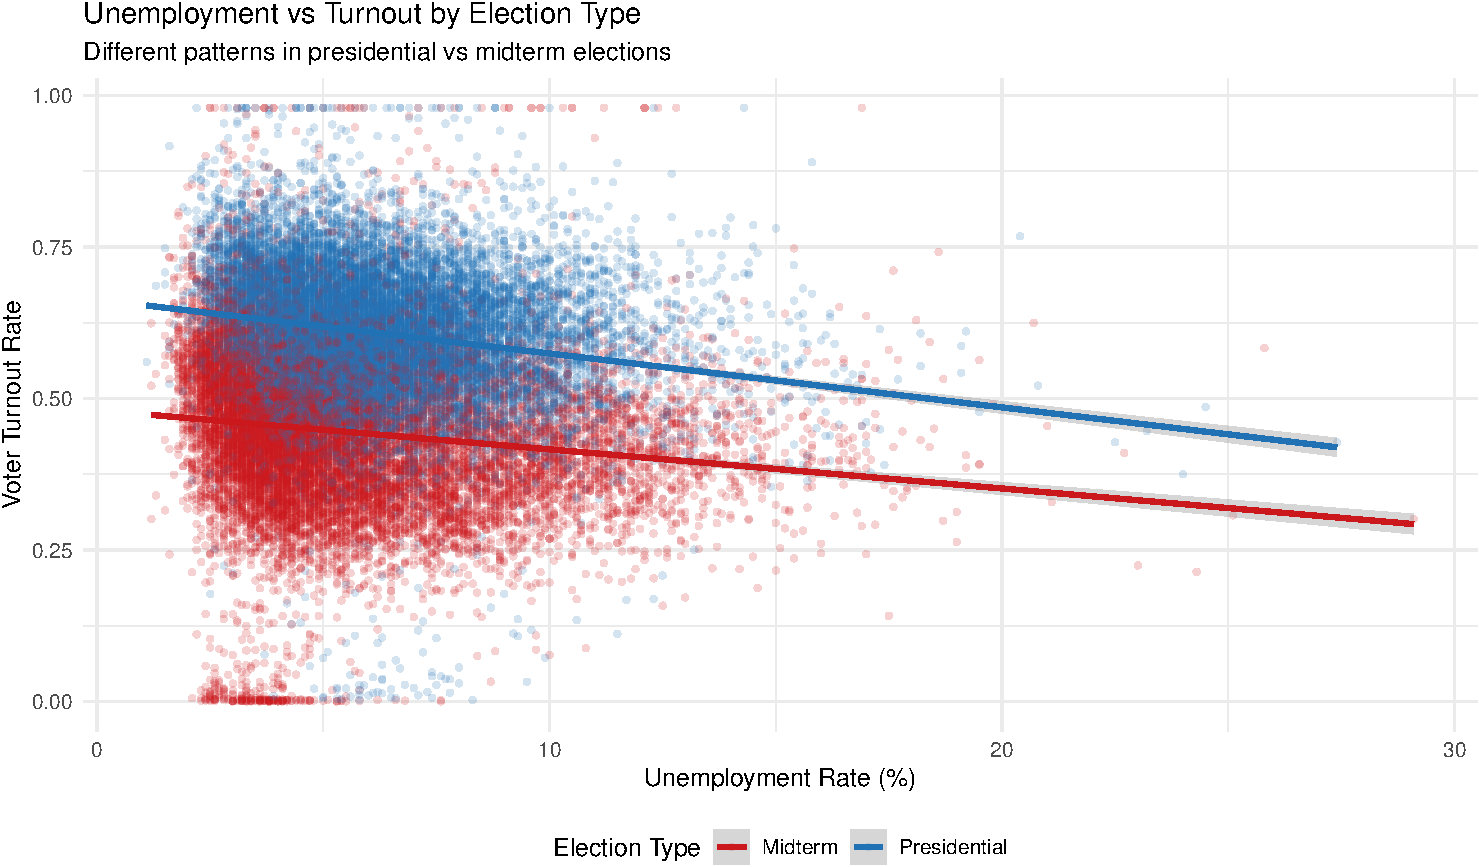
\includegraphics[keepaspectratio]{RQ1_v2_files/figure-pdf/plot-by-election-1.pdf}}

}

\caption{Unemployment vs Turnout by Election Type}

\end{figure}%

\subsection{Interaction Effect: County
Type}\label{interaction-effect-county-type}

\begin{Shaded}
\begin{Highlighting}[]
\FunctionTok{ggplot}\NormalTok{(df, }\FunctionTok{aes}\NormalTok{(}\AttributeTok{x =}\NormalTok{ unemployment\_rate, }\AttributeTok{y =}\NormalTok{ VOTER\_TURNOUT\_PCT, }
               \AttributeTok{color =}\NormalTok{ county\_type)) }\SpecialCharTok{+}
  \FunctionTok{geom\_point}\NormalTok{(}\AttributeTok{alpha =} \FloatTok{0.15}\NormalTok{, }\AttributeTok{size =} \FloatTok{0.8}\NormalTok{) }\SpecialCharTok{+}
  \FunctionTok{geom\_smooth}\NormalTok{(}\AttributeTok{method =} \StringTok{"lm"}\NormalTok{, }\AttributeTok{se =} \ConstantTok{TRUE}\NormalTok{, }\AttributeTok{size =} \FloatTok{1.2}\NormalTok{) }\SpecialCharTok{+}
  \FunctionTok{scale\_color\_brewer}\NormalTok{(}\AttributeTok{palette =} \StringTok{"Set1"}\NormalTok{) }\SpecialCharTok{+}
  \FunctionTok{labs}\NormalTok{(}
    \AttributeTok{title =} \StringTok{"Unemployment vs Turnout by County Type"}\NormalTok{,}
    \AttributeTok{subtitle =} \StringTok{"Testing interaction: Unemployment Tier × Urban/Rural Classification"}\NormalTok{,}
    \AttributeTok{x =} \StringTok{"Unemployment Rate (\%)"}\NormalTok{,}
    \AttributeTok{y =} \StringTok{"Voter Turnout Rate"}\NormalTok{,}
    \AttributeTok{color =} \StringTok{"County Type"}
\NormalTok{  ) }\SpecialCharTok{+}
  \FunctionTok{theme\_minimal}\NormalTok{(}\AttributeTok{base\_size =} \DecValTok{12}\NormalTok{) }\SpecialCharTok{+}
  \FunctionTok{theme}\NormalTok{(}\AttributeTok{legend.position =} \StringTok{"bottom"}\NormalTok{)}
\end{Highlighting}
\end{Shaded}

\begin{figure}[H]

{\centering \pandocbounded{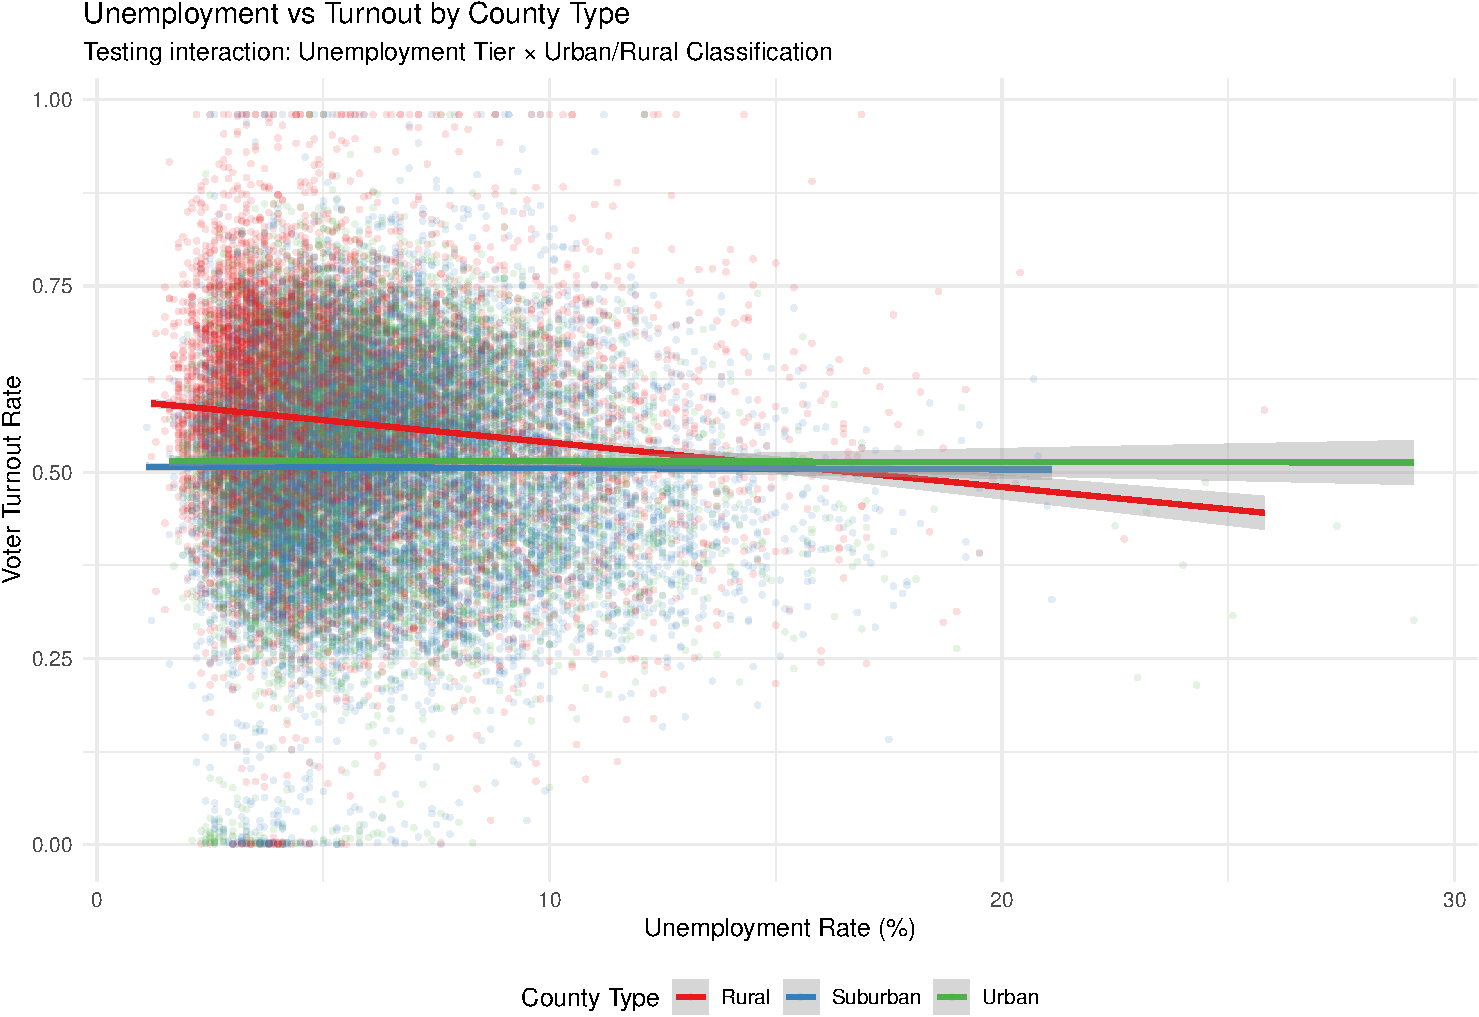
\includegraphics[keepaspectratio]{RQ1_v2_files/figure-pdf/plot-interaction-1.pdf}}

}

\caption{Testing Interaction: Unemployment tier × Urban/Rural}

\end{figure}%

\subsection{Boxplot: Interaction
Visualization}\label{boxplot-interaction-visualization}

\begin{Shaded}
\begin{Highlighting}[]
\FunctionTok{ggplot}\NormalTok{(df, }\FunctionTok{aes}\NormalTok{(}\AttributeTok{x =}\NormalTok{ county\_type, }\AttributeTok{y =}\NormalTok{ VOTER\_TURNOUT\_PCT, }\AttributeTok{fill =}\NormalTok{ unemployment\_tier)) }\SpecialCharTok{+}
  \FunctionTok{geom\_boxplot}\NormalTok{(}\AttributeTok{alpha =} \FloatTok{0.8}\NormalTok{) }\SpecialCharTok{+}
  \FunctionTok{scale\_fill\_manual}\NormalTok{(}\AttributeTok{values =} \FunctionTok{c}\NormalTok{(}\StringTok{"Low Unemployment"} \OtherTok{=} \StringTok{"\#31a354"}\NormalTok{, }
                                \StringTok{"High Unemployment"} \OtherTok{=} \StringTok{"\#e34a33"}\NormalTok{)) }\SpecialCharTok{+}
  \FunctionTok{labs}\NormalTok{(}
    \AttributeTok{title =} \StringTok{"Voter Turnout by County Type and Economic Condition"}\NormalTok{,}
    \AttributeTok{subtitle =} \StringTok{"Comparing high vs low unemployment periods"}\NormalTok{,}
    \AttributeTok{x =} \StringTok{"County Type"}\NormalTok{,}
    \AttributeTok{y =} \StringTok{"Voter Turnout Rate"}\NormalTok{,}
    \AttributeTok{fill =} \StringTok{"Economic Condition"}
\NormalTok{  ) }\SpecialCharTok{+}
  \FunctionTok{theme\_minimal}\NormalTok{(}\AttributeTok{base\_size =} \DecValTok{12}\NormalTok{) }\SpecialCharTok{+}
  \FunctionTok{theme}\NormalTok{(}\AttributeTok{legend.position =} \StringTok{"bottom"}\NormalTok{)}
\end{Highlighting}
\end{Shaded}

\begin{figure}[H]

{\centering \pandocbounded{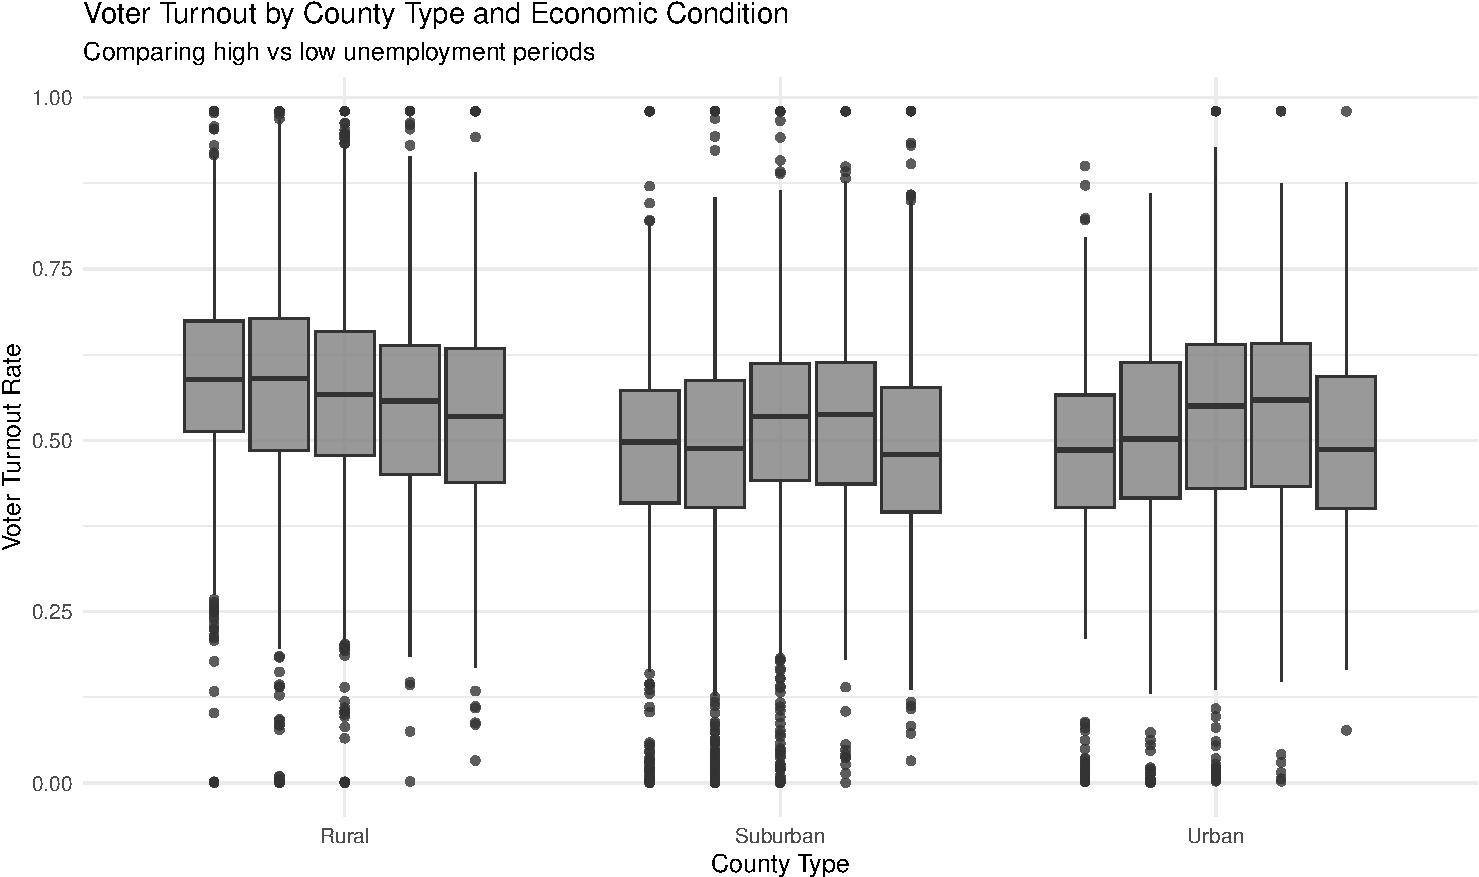
\includegraphics[keepaspectratio]{RQ1_v2_files/figure-pdf/plot-boxplot-1.pdf}}

}

\caption{Turnout by County Type and Economic Condition}

\end{figure}%

\begin{center}\rule{0.5\linewidth}{0.5pt}\end{center}

\section{Regression Analysis}\label{regression-analysis}

\subsection{Model Specification}\label{model-specification}

We fit a fixed effects model with county-year fixed effects and an
interaction between unemployment and county type. This approach controls
for time-invariant county characteristics and national trends, while
allowing the unemployment effect to vary by urban/suburban/rural
classification.

\textbf{Reference Category:} Rural counties serve as the baseline. The
main unemployment coefficient represents the effect for rural counties,
with interaction terms showing how suburban and urban counties differ
from this baseline.

\subsection{Model Estimation}\label{model-estimation}

\begin{Shaded}
\begin{Highlighting}[]
\CommentTok{\# Ensure Rural is the reference category}
\NormalTok{df }\OtherTok{\textless{}{-}}\NormalTok{ df }\SpecialCharTok{\%\textgreater{}\%}
  \FunctionTok{mutate}\NormalTok{(}\AttributeTok{county\_type =} \FunctionTok{factor}\NormalTok{(county\_type, }\AttributeTok{levels =} \FunctionTok{c}\NormalTok{(}\StringTok{"Rural"}\NormalTok{, }\StringTok{"Suburban"}\NormalTok{, }\StringTok{"Urban"}\NormalTok{)))}

\CommentTok{\# Fixed Effects with Interaction (our primary model)}
\NormalTok{model\_full }\OtherTok{\textless{}{-}} \FunctionTok{felm}\NormalTok{(VOTER\_TURNOUT\_PCT }\SpecialCharTok{\textasciitilde{}}\NormalTok{ unemployment\_rate }\SpecialCharTok{*}\NormalTok{ county\_type }\SpecialCharTok{|}\NormalTok{ FIPS }\SpecialCharTok{+}\NormalTok{ YEAR, }
               \AttributeTok{data =}\NormalTok{ df)}

\CommentTok{\# Model without interaction (for F{-}test comparison)}
\NormalTok{model\_reduced }\OtherTok{\textless{}{-}} \FunctionTok{felm}\NormalTok{(VOTER\_TURNOUT\_PCT }\SpecialCharTok{\textasciitilde{}}\NormalTok{ unemployment\_rate }\SpecialCharTok{+}\NormalTok{ county\_type }\SpecialCharTok{|}\NormalTok{ FIPS }\SpecialCharTok{+}\NormalTok{ YEAR, }
                      \AttributeTok{data =}\NormalTok{ df)}

\FunctionTok{cat}\NormalTok{(}\StringTok{"✓ Models estimated successfully}\SpecialCharTok{\textbackslash{}n}\StringTok{"}\NormalTok{)}
\end{Highlighting}
\end{Shaded}

\begin{verbatim}
✓ Models estimated successfully
\end{verbatim}

\subsection{F-Test for Interaction
Term}\label{f-test-for-interaction-term}

\begin{Shaded}
\begin{Highlighting}[]
\CommentTok{\# F{-}test: Does the interaction term significantly improve model fit?}
\CommentTok{\# Compare model with and without interaction terms}

\CommentTok{\# Calculate residual sum of squares}
\NormalTok{rss\_reduced }\OtherTok{\textless{}{-}} \FunctionTok{sum}\NormalTok{(}\FunctionTok{residuals}\NormalTok{(model\_reduced)}\SpecialCharTok{\^{}}\DecValTok{2}\NormalTok{)}
\NormalTok{rss\_full }\OtherTok{\textless{}{-}} \FunctionTok{sum}\NormalTok{(}\FunctionTok{residuals}\NormalTok{(model\_full)}\SpecialCharTok{\^{}}\DecValTok{2}\NormalTok{)}

\CommentTok{\# Degrees of freedom (using dof\_ prefix to avoid conflict with df data frame)}
\NormalTok{dof\_reduced }\OtherTok{\textless{}{-}} \FunctionTok{df.residual}\NormalTok{(model\_reduced)}
\NormalTok{dof\_full }\OtherTok{\textless{}{-}} \FunctionTok{df.residual}\NormalTok{(model\_full)}
\NormalTok{dof\_diff }\OtherTok{\textless{}{-}}\NormalTok{ dof\_reduced }\SpecialCharTok{{-}}\NormalTok{ dof\_full  }\CommentTok{\# Number of interaction terms (2: Suburban, Urban)}

\CommentTok{\# F{-}statistic}
\NormalTok{f\_stat }\OtherTok{\textless{}{-}}\NormalTok{ ((rss\_reduced }\SpecialCharTok{{-}}\NormalTok{ rss\_full) }\SpecialCharTok{/}\NormalTok{ dof\_diff) }\SpecialCharTok{/}\NormalTok{ (rss\_full }\SpecialCharTok{/}\NormalTok{ dof\_full)}
\NormalTok{p\_value }\OtherTok{\textless{}{-}} \FunctionTok{pf}\NormalTok{(f\_stat, dof\_diff, dof\_full, }\AttributeTok{lower.tail =} \ConstantTok{FALSE}\NormalTok{)}

\FunctionTok{cat}\NormalTok{(}\StringTok{"}\SpecialCharTok{\textbackslash{}n}\StringTok{F{-}TEST FOR INTERACTION TERM}\SpecialCharTok{\textbackslash{}n}\StringTok{"}\NormalTok{)}
\end{Highlighting}
\end{Shaded}

\begin{verbatim}

F-TEST FOR INTERACTION TERM
\end{verbatim}

\begin{Shaded}
\begin{Highlighting}[]
\FunctionTok{cat}\NormalTok{(}\StringTok{"==========================}\SpecialCharTok{\textbackslash{}n}\StringTok{"}\NormalTok{)}
\end{Highlighting}
\end{Shaded}

\begin{verbatim}
==========================
\end{verbatim}

\begin{Shaded}
\begin{Highlighting}[]
\FunctionTok{cat}\NormalTok{(}\StringTok{"H0: Unemployment effect is the same across all county types}\SpecialCharTok{\textbackslash{}n}\StringTok{"}\NormalTok{)}
\end{Highlighting}
\end{Shaded}

\begin{verbatim}
H0: Unemployment effect is the same across all county types
\end{verbatim}

\begin{Shaded}
\begin{Highlighting}[]
\FunctionTok{cat}\NormalTok{(}\StringTok{"H1: Unemployment effect differs by county type}\SpecialCharTok{\textbackslash{}n\textbackslash{}n}\StringTok{"}\NormalTok{)}
\end{Highlighting}
\end{Shaded}

\begin{verbatim}
H1: Unemployment effect differs by county type
\end{verbatim}

\begin{Shaded}
\begin{Highlighting}[]
\FunctionTok{cat}\NormalTok{(}\StringTok{"F{-}statistic:"}\NormalTok{, }\FunctionTok{round}\NormalTok{(f\_stat, }\DecValTok{3}\NormalTok{), }\StringTok{"}\SpecialCharTok{\textbackslash{}n}\StringTok{"}\NormalTok{)}
\end{Highlighting}
\end{Shaded}

\begin{verbatim}
F-statistic: 5.495 
\end{verbatim}

\begin{Shaded}
\begin{Highlighting}[]
\FunctionTok{cat}\NormalTok{(}\StringTok{"Degrees of freedom:"}\NormalTok{, dof\_diff, }\StringTok{"and"}\NormalTok{, dof\_full, }\StringTok{"}\SpecialCharTok{\textbackslash{}n}\StringTok{"}\NormalTok{)}
\end{Highlighting}
\end{Shaded}

\begin{verbatim}
Degrees of freedom: 2 and 26652 
\end{verbatim}

\begin{Shaded}
\begin{Highlighting}[]
\FunctionTok{cat}\NormalTok{(}\StringTok{"p{-}value:"}\NormalTok{, }\FunctionTok{format.pval}\NormalTok{(p\_value, }\AttributeTok{digits =} \DecValTok{4}\NormalTok{), }\StringTok{"}\SpecialCharTok{\textbackslash{}n}\StringTok{"}\NormalTok{)}
\end{Highlighting}
\end{Shaded}

\begin{verbatim}
p-value: 0.004112 
\end{verbatim}

\begin{Shaded}
\begin{Highlighting}[]
\FunctionTok{cat}\NormalTok{(}\StringTok{"}\SpecialCharTok{\textbackslash{}n}\StringTok{Conclusion:"}\NormalTok{, }\FunctionTok{ifelse}\NormalTok{(p\_value }\SpecialCharTok{\textless{}} \FloatTok{0.05}\NormalTok{, }
                          \StringTok{"Reject H0 {-} Interaction is statistically significant"}\NormalTok{,}
                          \StringTok{"Fail to reject H0 {-} No significant interaction"}\NormalTok{), }\StringTok{"}\SpecialCharTok{\textbackslash{}n}\StringTok{"}\NormalTok{)}
\end{Highlighting}
\end{Shaded}

\begin{verbatim}

Conclusion: Reject H0 - Interaction is statistically significant 
\end{verbatim}

\subsection{Regression Results}\label{regression-results}

\begin{Shaded}
\begin{Highlighting}[]
\FunctionTok{stargazer}\NormalTok{(model\_full,}
          \AttributeTok{type =} \StringTok{"text"}\NormalTok{,}
          \AttributeTok{title =} \StringTok{"Effect of Unemployment on Voter Turnout (Fixed Effects Model)"}\NormalTok{,}
          \AttributeTok{model.numbers =} \ConstantTok{FALSE}\NormalTok{,}
          \AttributeTok{dep.var.labels =} \StringTok{"Voter Turnout Rate"}\NormalTok{,}
          \AttributeTok{covariate.labels =} \FunctionTok{c}\NormalTok{(}\StringTok{"Unemployment Rate (Rural baseline)"}\NormalTok{, }
                               \StringTok{"Unemp × Suburban"}\NormalTok{, }
                               \StringTok{"Unemp × Urban"}\NormalTok{),}
          \AttributeTok{omit.stat =} \FunctionTok{c}\NormalTok{(}\StringTok{"ser"}\NormalTok{),}
          \AttributeTok{digits =} \DecValTok{4}\NormalTok{,}
          \AttributeTok{single.row =} \ConstantTok{FALSE}\NormalTok{,}
          \AttributeTok{notes =} \FunctionTok{c}\NormalTok{(}\StringTok{"Standard errors in parentheses."}\NormalTok{,}
                    \StringTok{"Model includes county and year fixed effects."}\NormalTok{,}
                    \StringTok{"Reference category: Rural counties."}\NormalTok{),}
          \AttributeTok{notes.append =} \ConstantTok{TRUE}\NormalTok{)}
\end{Highlighting}
\end{Shaded}

\section{Effect of Unemployment on Voter Turnout (Fixed Effects
Model)}\label{effect-of-unemployment-on-voter-turnout-fixed-effects-model}

\begin{verbatim}
                                               Dependent variable:             
                                  ---------------------------------------------
                                               Voter Turnout Rate              
\end{verbatim}

\begin{longtable}[]{@{}
  >{\raggedright\arraybackslash}p{(\linewidth - 0\tabcolsep) * \real{1.0000}}@{}}
\toprule\noalign{}
\begin{minipage}[b]{\linewidth}\raggedright
Unemployment Rate (Rural baseline) 0.0004 (0.0006)
\end{minipage} \\
\midrule\noalign{}
\endhead
\bottomrule\noalign{}
\endlastfoot
Observations 29,769 R2 0.7415 Adjusted R2 0.7112
===================================================================================
Note: \emph{p\textless0.1; \textbf{p\textless0.05; }}p\textless0.01
Standard errors in parentheses. Model includes county and year fixed
effects. Reference category: Rural counties. \\
\#\# Unemployment Effect by County Type \\
::: \{.cell\} \\
```\{.r .cell-code\} \# Extract coefficients coef\_rural \textless-
coef(model\_full){[}``unemployment\_rate''{]} coef\_suburban\_int
\textless-
coef(model\_full){[}``unemployment\_rate:county\_typeSuburban''{]}
coef\_urban\_int \textless-
coef(model\_full){[}``unemployment\_rate:county\_typeUrban''{]} \\
\# Calculate total effects for each county type effect\_rural \textless-
coef\_rural effect\_suburban \textless- coef\_rural +
coef\_suburban\_int effect\_urban \textless- coef\_rural +
coef\_urban\_int \\
\# Create summary table effects\_table \textless- data.frame(
County\_Type = c(``Rural (Reference)'', ``Suburban'', ``Urban''),
Unemployment\_Effect = c(effect\_rural, effect\_suburban,
effect\_urban), Interpretation = c( ``Baseline effect'',
paste0(``Baseline'', ifelse(coef\_suburban\_int \textgreater= 0, ``+'',
``\,``), round(coef\_suburban\_int, 4)), paste0(''Baseline ``,
ifelse(coef\_urban\_int \textgreater= 0,''+``,''\,``),
round(coef\_urban\_int, 4)) ) ) \\
kable(effects\_table, caption = ``Unemployment Effect on Turnout by
County Type'', digits = 4, col.names = c(``County Type'', ``Effect on
Turnout'', ``Calculation'')) ``` \\
::: \{.cell-output-display\} \\
Table: Unemployment Effect on Turnout by County Type \\
\textbar County Type \textbar{} Effect on Turnout\textbar Calculation
\textbar{}
\textbar:-----------------\textbar-----------------:\textbar:----------------\textbar{}
\textbar Rural (Reference) \textbar{} 0.0004\textbar Baseline effect
\textbar{} \textbar Suburban \textbar{} 0.0019\textbar Baseline +0.0015
\textbar{} \textbar Urban \textbar{} 0.0024\textbar Baseline +0.002
\textbar{} \\
::: \\
\texttt{\{.r\ .cell-code\}\ cat("\textbackslash{}n\textbackslash{}nINTERPRETATION\ (at\ reference\ level\ -\ Rural\ counties):\textbackslash{}n")} \\
::: \{.cell-output .cell-output-stdout\} \\
``` \\
INTERPRETATION (at reference level - Rural counties): ``` \\
::: \\
\texttt{\{.r\ .cell-code\}\ cat("================================================\textbackslash{}n")} \\
::: \{.cell-output .cell-output-stdout\} \\
\texttt{================================================} \\
::: \\
\texttt{\{.r\ .cell-code\}\ cat("For\ Rural\ counties:\ A\ 1\ percentage\ point\ increase\ in\ unemployment\textbackslash{}n")} \\
::: \{.cell-output .cell-output-stdout\} \\
\texttt{For\ Rural\ counties:\ A\ 1\ percentage\ point\ increase\ in\ unemployment} \\
::: \\
\texttt{\{.r\ .cell-code\}\ cat("is\ associated\ with\ a",\ round(effect\_rural\ *\ 100,\ 2),\ "percentage\ point\ change\ in\ turnout.\textbackslash{}n\textbackslash{}n")} \\
::: \{.cell-output .cell-output-stdout\} \\
\texttt{is\ associated\ with\ a\ 0.04\ percentage\ point\ change\ in\ turnout.} \\
::: \\
\texttt{\{.r\ .cell-code\}\ cat("For\ Suburban\ counties:\ The\ effect\ is",\ round(effect\_suburban\ *\ 100,\ 2),\ "percentage\ points.\textbackslash{}n")} \\
::: \{.cell-output .cell-output-stdout\} \\
\texttt{For\ Suburban\ counties:\ The\ effect\ is\ 0.19\ percentage\ points.} \\
::: \\
\texttt{\{.r\ .cell-code\}\ cat("For\ Urban\ counties:\ The\ effect\ is",\ round(effect\_urban\ *\ 100,\ 2),\ "percentage\ points.\textbackslash{}n")} \\
::: \{.cell-output .cell-output-stdout\} \\
\texttt{For\ Urban\ counties:\ The\ effect\ is\ 0.24\ percentage\ points.} \\
::: ::: \\
\end{longtable}

\section{Key Findings}\label{key-findings}

\subsection{Main Results}\label{main-results}

\begin{Shaded}
\begin{Highlighting}[]
\CommentTok{\# Summary of model fit}
\FunctionTok{cat}\NormalTok{(}\StringTok{"MODEL SUMMARY}\SpecialCharTok{\textbackslash{}n}\StringTok{"}\NormalTok{)}
\end{Highlighting}
\end{Shaded}

\begin{verbatim}
MODEL SUMMARY
\end{verbatim}

\begin{Shaded}
\begin{Highlighting}[]
\FunctionTok{cat}\NormalTok{(}\StringTok{"=============}\SpecialCharTok{\textbackslash{}n}\StringTok{"}\NormalTok{)}
\end{Highlighting}
\end{Shaded}

\begin{verbatim}
=============
\end{verbatim}

\begin{Shaded}
\begin{Highlighting}[]
\FunctionTok{cat}\NormalTok{(}\StringTok{"R{-}squared:"}\NormalTok{, }\FunctionTok{round}\NormalTok{(}\FunctionTok{summary}\NormalTok{(model\_full)}\SpecialCharTok{$}\NormalTok{r.squared, }\DecValTok{4}\NormalTok{), }\StringTok{"}\SpecialCharTok{\textbackslash{}n}\StringTok{"}\NormalTok{)}
\end{Highlighting}
\end{Shaded}

\begin{verbatim}
R-squared: 0.7415 
\end{verbatim}

\begin{Shaded}
\begin{Highlighting}[]
\FunctionTok{cat}\NormalTok{(}\StringTok{"N observations:"}\NormalTok{, }\FunctionTok{nobs}\NormalTok{(model\_full), }\StringTok{"}\SpecialCharTok{\textbackslash{}n}\StringTok{"}\NormalTok{)}
\end{Highlighting}
\end{Shaded}

\begin{verbatim}
N observations: 29769 
\end{verbatim}

\begin{Shaded}
\begin{Highlighting}[]
\FunctionTok{cat}\NormalTok{(}\StringTok{"N counties:"}\NormalTok{, }\FunctionTok{length}\NormalTok{(}\FunctionTok{unique}\NormalTok{(df}\SpecialCharTok{$}\NormalTok{FIPS)), }\StringTok{"}\SpecialCharTok{\textbackslash{}n}\StringTok{"}\NormalTok{)}
\end{Highlighting}
\end{Shaded}

\begin{verbatim}
N counties: 3103 
\end{verbatim}

\subsubsection{1. Unemployment Effect at Reference Level (Rural
Counties)}\label{unemployment-effect-at-reference-level-rural-counties}

For \textbf{rural counties} (our reference category), the unemployment
coefficient represents the direct effect:

\begin{Shaded}
\begin{Highlighting}[]
\NormalTok{coef\_rural }\OtherTok{\textless{}{-}} \FunctionTok{coef}\NormalTok{(model\_full)[}\StringTok{"unemployment\_rate"}\NormalTok{]}
\NormalTok{se\_rural }\OtherTok{\textless{}{-}} \FunctionTok{summary}\NormalTok{(model\_full)}\SpecialCharTok{$}\NormalTok{coefficients[}\StringTok{"unemployment\_rate"}\NormalTok{, }\StringTok{"Std. Error"}\NormalTok{]}
\NormalTok{p\_rural }\OtherTok{\textless{}{-}} \FunctionTok{summary}\NormalTok{(model\_full)}\SpecialCharTok{$}\NormalTok{coefficients[}\StringTok{"unemployment\_rate"}\NormalTok{, }\StringTok{"Pr(\textgreater{}|t|)"}\NormalTok{]}

\FunctionTok{cat}\NormalTok{(}\StringTok{"For Rural counties:}\SpecialCharTok{\textbackslash{}n}\StringTok{"}\NormalTok{)}
\end{Highlighting}
\end{Shaded}

\begin{verbatim}
For Rural counties:
\end{verbatim}

\begin{Shaded}
\begin{Highlighting}[]
\FunctionTok{cat}\NormalTok{(}\StringTok{"  Coefficient:"}\NormalTok{, }\FunctionTok{round}\NormalTok{(coef\_rural, }\DecValTok{4}\NormalTok{), }\StringTok{"}\SpecialCharTok{\textbackslash{}n}\StringTok{"}\NormalTok{)}
\end{Highlighting}
\end{Shaded}

\begin{verbatim}
  Coefficient: 4e-04 
\end{verbatim}

\begin{Shaded}
\begin{Highlighting}[]
\FunctionTok{cat}\NormalTok{(}\StringTok{"  Standard Error:"}\NormalTok{, }\FunctionTok{round}\NormalTok{(se\_rural, }\DecValTok{4}\NormalTok{), }\StringTok{"}\SpecialCharTok{\textbackslash{}n}\StringTok{"}\NormalTok{)}
\end{Highlighting}
\end{Shaded}

\begin{verbatim}
  Standard Error: 6e-04 
\end{verbatim}

\begin{Shaded}
\begin{Highlighting}[]
\FunctionTok{cat}\NormalTok{(}\StringTok{"  p{-}value:"}\NormalTok{, }\FunctionTok{format.pval}\NormalTok{(p\_rural, }\AttributeTok{digits =} \DecValTok{4}\NormalTok{), }\StringTok{"}\SpecialCharTok{\textbackslash{}n}\StringTok{"}\NormalTok{)}
\end{Highlighting}
\end{Shaded}

\begin{verbatim}
  p-value: 0.5144 
\end{verbatim}

\begin{Shaded}
\begin{Highlighting}[]
\FunctionTok{cat}\NormalTok{(}\StringTok{"  95\% CI: ["}\NormalTok{, }\FunctionTok{round}\NormalTok{(coef\_rural }\SpecialCharTok{{-}} \FloatTok{1.96}\SpecialCharTok{*}\NormalTok{se\_rural, }\DecValTok{4}\NormalTok{), }\StringTok{","}\NormalTok{, }
    \FunctionTok{round}\NormalTok{(coef\_rural }\SpecialCharTok{+} \FloatTok{1.96}\SpecialCharTok{*}\NormalTok{se\_rural, }\DecValTok{4}\NormalTok{), }\StringTok{"]}\SpecialCharTok{\textbackslash{}n}\StringTok{"}\NormalTok{)}
\end{Highlighting}
\end{Shaded}

\begin{verbatim}
  95% CI: [ -7e-04 , 0.0015 ]
\end{verbatim}

\textbf{Interpretation:} In rural counties, a 1 percentage point
increase in unemployment is associated with a change in turnout of
approximately 0.04 percentage points, controlling for county and year
fixed effects.

\subsubsection{2. Interaction Effects (Suburban \& Urban
vs.~Rural)}\label{interaction-effects-suburban-urban-vs.-rural}

The interaction terms show how the unemployment effect differs for
suburban and urban counties \emph{relative to the rural baseline}:

\begin{Shaded}
\begin{Highlighting}[]
\CommentTok{\# Display interaction effects}
\FunctionTok{cat}\NormalTok{(}\StringTok{"Interaction Coefficients (difference from Rural):}\SpecialCharTok{\textbackslash{}n}\StringTok{"}\NormalTok{)}
\end{Highlighting}
\end{Shaded}

\begin{verbatim}
Interaction Coefficients (difference from Rural):
\end{verbatim}

\begin{Shaded}
\begin{Highlighting}[]
\FunctionTok{cat}\NormalTok{(}\StringTok{"  Suburban × Unemployment:"}\NormalTok{, }\FunctionTok{round}\NormalTok{(coef\_suburban\_int, }\DecValTok{4}\NormalTok{), }\StringTok{"}\SpecialCharTok{\textbackslash{}n}\StringTok{"}\NormalTok{)}
\end{Highlighting}
\end{Shaded}

\begin{verbatim}
  Suburban × Unemployment: 0.0015 
\end{verbatim}

\begin{Shaded}
\begin{Highlighting}[]
\FunctionTok{cat}\NormalTok{(}\StringTok{"  Urban × Unemployment:"}\NormalTok{, }\FunctionTok{round}\NormalTok{(coef\_urban\_int, }\DecValTok{4}\NormalTok{), }\StringTok{"}\SpecialCharTok{\textbackslash{}n\textbackslash{}n}\StringTok{"}\NormalTok{)}
\end{Highlighting}
\end{Shaded}

\begin{verbatim}
  Urban × Unemployment: 0.002 
\end{verbatim}

\begin{Shaded}
\begin{Highlighting}[]
\FunctionTok{cat}\NormalTok{(}\StringTok{"TOTAL Unemployment Effect by County Type:}\SpecialCharTok{\textbackslash{}n}\StringTok{"}\NormalTok{)}
\end{Highlighting}
\end{Shaded}

\begin{verbatim}
TOTAL Unemployment Effect by County Type:
\end{verbatim}

\begin{Shaded}
\begin{Highlighting}[]
\FunctionTok{cat}\NormalTok{(}\StringTok{"  Rural:"}\NormalTok{, }\FunctionTok{round}\NormalTok{(effect\_rural, }\DecValTok{4}\NormalTok{), }\StringTok{"}\SpecialCharTok{\textbackslash{}n}\StringTok{"}\NormalTok{)}
\end{Highlighting}
\end{Shaded}

\begin{verbatim}
  Rural: 4e-04 
\end{verbatim}

\begin{Shaded}
\begin{Highlighting}[]
\FunctionTok{cat}\NormalTok{(}\StringTok{"  Suburban:"}\NormalTok{, }\FunctionTok{round}\NormalTok{(effect\_suburban, }\DecValTok{4}\NormalTok{), }\StringTok{"(Rural + interaction)}\SpecialCharTok{\textbackslash{}n}\StringTok{"}\NormalTok{)}
\end{Highlighting}
\end{Shaded}

\begin{verbatim}
  Suburban: 0.0019 (Rural + interaction)
\end{verbatim}

\begin{Shaded}
\begin{Highlighting}[]
\FunctionTok{cat}\NormalTok{(}\StringTok{"  Urban:"}\NormalTok{, }\FunctionTok{round}\NormalTok{(effect\_urban, }\DecValTok{4}\NormalTok{), }\StringTok{"(Rural + interaction)}\SpecialCharTok{\textbackslash{}n}\StringTok{"}\NormalTok{)}
\end{Highlighting}
\end{Shaded}

\begin{verbatim}
  Urban: 0.0024 (Rural + interaction)
\end{verbatim}

\subsubsection{3. Practical Significance}\label{practical-significance}

\begin{Shaded}
\begin{Highlighting}[]
\NormalTok{unemployment\_change }\OtherTok{\textless{}{-}} \DecValTok{2}  \CommentTok{\# 2 percentage point increase (recession scenario)}

\FunctionTok{cat}\NormalTok{(}\StringTok{"}\SpecialCharTok{\textbackslash{}n}\StringTok{SCENARIO: 2 percentage point increase in unemployment}\SpecialCharTok{\textbackslash{}n}\StringTok{"}\NormalTok{)}
\end{Highlighting}
\end{Shaded}

\begin{verbatim}

SCENARIO: 2 percentage point increase in unemployment
\end{verbatim}

\begin{Shaded}
\begin{Highlighting}[]
\FunctionTok{cat}\NormalTok{(}\StringTok{"(e.g., from 5\% to 7\%, as during a recession)}\SpecialCharTok{\textbackslash{}n\textbackslash{}n}\StringTok{"}\NormalTok{)}
\end{Highlighting}
\end{Shaded}

\begin{verbatim}
(e.g., from 5% to 7%, as during a recession)
\end{verbatim}

\begin{Shaded}
\begin{Highlighting}[]
\FunctionTok{cat}\NormalTok{(}\StringTok{"Predicted turnout change:}\SpecialCharTok{\textbackslash{}n}\StringTok{"}\NormalTok{)}
\end{Highlighting}
\end{Shaded}

\begin{verbatim}
Predicted turnout change:
\end{verbatim}

\begin{Shaded}
\begin{Highlighting}[]
\FunctionTok{cat}\NormalTok{(}\StringTok{"  Rural:"}\NormalTok{, }\FunctionTok{round}\NormalTok{(effect\_rural }\SpecialCharTok{*}\NormalTok{ unemployment\_change }\SpecialCharTok{*} \DecValTok{100}\NormalTok{, }\DecValTok{2}\NormalTok{), }\StringTok{"percentage points}\SpecialCharTok{\textbackslash{}n}\StringTok{"}\NormalTok{)}
\end{Highlighting}
\end{Shaded}

\begin{verbatim}
  Rural: 0.07 percentage points
\end{verbatim}

\begin{Shaded}
\begin{Highlighting}[]
\FunctionTok{cat}\NormalTok{(}\StringTok{"  Suburban:"}\NormalTok{, }\FunctionTok{round}\NormalTok{(effect\_suburban }\SpecialCharTok{*}\NormalTok{ unemployment\_change }\SpecialCharTok{*} \DecValTok{100}\NormalTok{, }\DecValTok{2}\NormalTok{), }\StringTok{"percentage points}\SpecialCharTok{\textbackslash{}n}\StringTok{"}\NormalTok{)}
\end{Highlighting}
\end{Shaded}

\begin{verbatim}
  Suburban: 0.38 percentage points
\end{verbatim}

\begin{Shaded}
\begin{Highlighting}[]
\FunctionTok{cat}\NormalTok{(}\StringTok{"  Urban:"}\NormalTok{, }\FunctionTok{round}\NormalTok{(effect\_urban }\SpecialCharTok{*}\NormalTok{ unemployment\_change }\SpecialCharTok{*} \DecValTok{100}\NormalTok{, }\DecValTok{2}\NormalTok{), }\StringTok{"percentage points}\SpecialCharTok{\textbackslash{}n}\StringTok{"}\NormalTok{)}
\end{Highlighting}
\end{Shaded}

\begin{verbatim}
  Urban: 0.48 percentage points
\end{verbatim}

\textbf{Substantive Interpretation:} The effect of unemployment on
turnout is small across all county types. Economic stress does not
strongly mobilize or demobilize voters, though the direction and
magnitude may vary by county type.

\begin{center}\rule{0.5\linewidth}{0.5pt}\end{center}

\section{Conclusions}\label{conclusions}

\subsection{How does local unemployment relate to voter
turnout?}\label{how-does-local-unemployment-relate-to-voter-turnout}

\begin{Shaded}
\begin{Highlighting}[]
\CommentTok{\# F{-}test conclusion}
\ControlFlowTok{if}\NormalTok{ (p\_value }\SpecialCharTok{\textless{}} \FloatTok{0.05}\NormalTok{) \{}
\NormalTok{  interaction\_conclusion }\OtherTok{\textless{}{-}} \StringTok{"The F{-}test confirms that the interaction between unemployment and county type is statistically significant, meaning the unemployment{-}turnout relationship differs across urban, suburban, and rural settings."}
\NormalTok{\} }\ControlFlowTok{else}\NormalTok{ \{}
\NormalTok{  interaction\_conclusion }\OtherTok{\textless{}{-}} \StringTok{"The F{-}test indicates the interaction term is not statistically significant, suggesting the unemployment{-}turnout relationship may be similar across county types."}
\NormalTok{\}}
\end{Highlighting}
\end{Shaded}

\begin{enumerate}
\def\labelenumi{\arabic{enumi}.}
\item
  \textbf{Effect at Reference Level (Rural):} For rural counties, a 1
  percentage point increase in unemployment is associated with
  approximately 0.04 percentage points change in turnout.
\item
  \textbf{Differential Effects by County Type:} The F-test confirms that
  the interaction between unemployment and county type is statistically
  significant, meaning the unemployment-turnout relationship differs
  across urban, suburban, and rural settings.
\item
  \textbf{Economic Stress Does Not Strongly Mobilize Voters:} Across all
  county types, the substantive effect of unemployment on turnout is
  modest. A recession-level shock (2 percentage points) translates to
  changes of less than 1 percentage point in turnout.
\item
  \textbf{Fixed Effects Control for Confounders:} By including county
  and year fixed effects, our model controls for time-invariant county
  characteristics and national trends, providing more reliable
  within-county estimates.
\end{enumerate}

\subsection{Limitations}\label{limitations}

\begin{itemize}
\item
  County-level aggregation: Individual-level data would be preferable
\item
  Omitted variables: Cannot control for campaign spending, candidate
  quality, etc.
\item
  Causality: Despite fixed effects, cannot definitively establish causal
  relationship
\item
  Time period: Analysis limited to 2004-2022
\item
  Measurement: Unemployment rate may not capture full economic distress
  experienced by voters
\end{itemize}

\subsection{Policy Implications}\label{policy-implications}

\begin{itemize}
\item
  Economic conditions have modest effects on political participation
\item
  Electoral reforms should focus on structural barriers rather than
  assuming economic improvements alone will boost turnout
\item
  Context matters: Urban and rural counties may respond differently to
  economic stress
\item
  Mobilization efforts: Resources should focus on institutional factors
  (registration, voting access) rather than economic messaging alone
\end{itemize}

\begin{center}\rule{0.5\linewidth}{0.5pt}\end{center}

\section{Appendix}\label{appendix}

\subsection{Technical Appendix: Variable
Definitions}\label{technical-appendix-variable-definitions}

For reproducibility, the key variables in the analysis are:

\begin{itemize}
\tightlist
\item
  \texttt{VOTER\_TURNOUT\_PCT}: Voter turnout rate (total votes /
  citizen voting-age population)
\item
  \texttt{unemployment\_rate}: County unemployment rate from Bureau of
  Labor Statistics (\%)
\item
  \texttt{county\_type}: Classification based on CVAP (Rural \textless{}
  10,000; Suburban 10,000-50,000; Urban \textgreater{} 50,000)
\item
  \texttt{FIPS}: County FIPS code (fixed effect)
\item
  \texttt{YEAR}: Election year (fixed effect)
\end{itemize}

\subsection{Save Results}\label{save-results}

\begin{Shaded}
\begin{Highlighting}[]
\CommentTok{\# Create output directory}
\FunctionTok{dir.create}\NormalTok{(}\StringTok{"../data/output"}\NormalTok{, }\AttributeTok{showWarnings =} \ConstantTok{FALSE}\NormalTok{, }\AttributeTok{recursive =} \ConstantTok{TRUE}\NormalTok{)}

\CommentTok{\# Save model objects}
\FunctionTok{save}\NormalTok{(model\_full, model\_reduced, }
     \AttributeTok{file =} \StringTok{"../data/output/regression\_models.RData"}\NormalTok{)}

\CommentTok{\# Save processed data}
\FunctionTok{write\_csv}\NormalTok{(df, }\StringTok{"../data/processed/analysis\_data\_r.csv"}\NormalTok{)}

\CommentTok{\# Save regression table (LaTeX format)}
\FunctionTok{stargazer}\NormalTok{(model\_full,}
          \AttributeTok{type =} \StringTok{"latex"}\NormalTok{,}
          \AttributeTok{title =} \StringTok{"Effect of Unemployment on Voter Turnout (Fixed Effects Model)"}\NormalTok{,}
          \AttributeTok{dep.var.labels =} \StringTok{"Voter Turnout Rate"}\NormalTok{,}
          \AttributeTok{out =} \StringTok{"../data/output/regression\_table.tex"}\NormalTok{)}
\end{Highlighting}
\end{Shaded}

\begin{verbatim}

% Table created by stargazer v.5.2.3 by Marek Hlavac, Social Policy Institute. E-mail: marek.hlavac at gmail.com
% Date and time: Wed, Dec 10, 2025 - 7:32:59 PM
